\documentclass[USenglish,oneside,twocolumn]{article}
\usepackage{color}
\usepackage[hyphens]{url}
\usepackage{longtable}
\usepackage{graphicx}
\usepackage{enumitem}
\usepackage{pdfpages}
%\usepackage{hyperref}

\usepackage[utf8]{inputenc}%(only for the pdftex engine)
%\RequirePackage[no-math]{fontspec}%(only for the luatex or the xetex engine)
\usepackage[big]{dgruyter_NEW}
 
\DOI{foobar}

\cclogo{
\includegraphics{by-nc-nd.pdf}}

% Format a participant quotation.
\newcommand{\pquote}[2]{
\begin{quotation}
\noindent #1:~\textit{``#2''}
\end{quotation}
}
  
\begin{document}
 
  \author*[1]{Linda Lee}

  \author[2]{David Fifield}

  \author[3]{Nathan Malkin}

  \author[4]{Ganesh Iyer}

  \author[5]{Serge Egelman}
  
  \author[6]{David Wagner}

  \affil[1]{University of California Berkeley, E-mail: \mbox{lnl@cs.berkeley.edu}}

  \affil[2]{University of California Berkeley, E-mail: \mbox{fifield@cs.berkeley.edu}}

  \affil[3]{University of California Berkeley, E-mail: \mbox{nmalkin@cs.berkeley.edu}}

  \affil[4]{University of California Berkeley, E-mail: \mbox{ganesh.v@berkeley.edu}}
  
  \affil[5]{University of California Berkeley and International Computer Science Institute, E-mail: \mbox{egelman@cs.berkeley.edu}}
   
  \affil[6]{University of California Berkeley, E-mail: \mbox{daw@cs.berkeley.edu}}

  \title{\huge Tor's Usability for Censorship Circumvention}
  %Internet Freedom Made Easy: On Improving Tor’s Usability for Censorship Circumvention
  %Towards Usable Censorship Circumvention

  \runningtitle{Tor's Usability for Censorship Circumvention}

  %\subtitle{...}

  \begin{abstract}
{Tor has grown beyond its original purpose as an anonymity tool and has 
since become an important censorship circumvention tool. We conducted a series of 
experiments to improve the Tor launcher configuration interface, which configures network components
that circumvent censorship. A 16-participant experiment and interview
identifies common user struggles while circumventing censorship.
We use as feedback to redesign the configuration interface.
We test the impact of our
changes on 124 participants to find that our changes results in a significant reduction 
in the spent configuring a connection, while maintaining the same rate of success. We
conclude with recommendations for changes to the current configuration interface and discuss
alternative configuration processes with different balances of risk, automation, and user input.}
\end{abstract}
  \keywords{User Studies, Tor, Security, Censorship, Anonymity}
%  \classification[PACS]{}
 % \communicated{...}
 % \dedication{...}

  \journalname{Proceedings on Privacy Enhancing Technologies}
\DOI{Editor to enter DOI}
  \startpage{1}
  \received{..}
  \revised{..}
  \accepted{..}

  \journalyear{2015}
  \journalvolume{2015}
  \journalissue{2}

\maketitle

\section{Introduction}

Although Tor~\cite{dingledine2004tor} was not designed to be a censorship circumvention tool, users started
using it as one, since Tor's anonymizing functionality also circumvented censorship. In fact, some countries unsuccessfully attempt to block Tor for this reason~\cite{winter2012great}. Today, Tor's network of unlisted relays and various methods of obfuscation making it a viable censorship circumvention tool even in the face of nation-state level adversaries.
 
To our knowledge, this is the first user study investigating the usability of Tor as a 
censorship circumvention tool. We believe that this is a great opportunity for user research, both for investigating a case study of investigating the usability of a censorship circumvention tool, and also to help current Tor users censorship circumvention more easily. Not only will this allow for easier censorship circumvention, users who use tor will be provided with extra security features that other censorship circumvention tools do not provide, such as anonymity. Additionally, increasing the adoption of Tor as a censorship circumvention tool benefits other users who use Tor as an anonymity system by increasing the number of overall users on the Tor network~\cite{dingledine2006anonymity}. 

Our study consists of two user studies set in three simulated censorship environments 
of varying levels of difficulty to circumvent. The mild, intermediate, and comprehensive 
environments required participants to connect, configure manually with default settings
and recommendations, and to configure manually without using defaults or recommendations. 
In both experiments, participants are informed that they are being censored, and that their 
goal is to reach a censored website by circumventing the censorship environment through
configuring Tor Browser. 

The first user study is a small-scale, one-on-one experiment that collected 
behavioral patterns and failure cases with the interface through user observations
and interviews(Section~\ref{sec:qualitative}). This feedback was used to make changes to the interface (Section~\ref{redesign}). The second user study is a large-scale, data-centric user study
that collected data on user interactions with the interface to quantify the impact of the design changes (Section~\ref{quantitative}).

Our study finds that that users had difficulty in answering technical questions, feel unqualified to make technical choices, and cannot tell why their connection is failing. We made ten design changes that aimed to provide additional feedback, unburden the user, and build a user's understanding of the process. Our changes decreased the time participants spent configuring their connections, with no decrease in success rates. We conclude with a recommendation of changes that we believe will increase the usability of Tor Browser's configuration interface. 

\section{Related Work} 
There have been three published user studies on Tor. Clark et. al examined various deployment
options for Tor Browser, such as Vidalia, Privoxy, Torbutton, and Foxyproxy, and found that none of them 
were satisfactory from a usability perspective~\cite{clark2007usability}. Fabian et. al show that Tor's added
latency~\cite{dingledine2009performance} causes users
to be frustrated, cancel requests more often, and prevents user adoption~\cite{fabian2010privately}. 
Norcie et. al found found that 
64\% of users are unable to continue with installation or browsing at least once due to difficulties~\cite{norcie2012eliminating}. 

There have been been no published usability evaluations of
Tor Browser since the 4.0 series, which introduced radical UI changes. 
The most recent usability effort is an unpublished pilot study  by Lee and Fifield~\cite {uxsprint} 
that tests the download, install, and  user interface of Tor Browser.  This study uncovered a number of issues~\cite{uxsprint2015-tickets}. Changes made are reflected in series 5.1 and later. 

Previous user studies have not focused on specific features in isolation, while we choose to focus our study on 
the configuration interface. The configuration interface guides users through setting up network components required to circumvent censorship. 
This study examines that interface, and effectively, the usability of Tor as a censorship circumvention tool. 

\section{Circumvention and Tor}

Censors of the Internet typically seek to block certain network resources such as websites.
They use various technical means, for example falsifying DNS responses,
blocking IP addresses, filtering keywords, and detecting protocols by deep packet inspection.
Internet users, naturally, try to evade a censor's blocks,
also employing a variety of technical means.

Tor is an anonymity network that has also grown into
a role as a vehicle for censorship circumvention.
Tor routes user traffic through a random series of relays
in a way that makes it difficult for an observer to connect source and destination.
Tor, in its native form, is easy for censors to block,
because the list of relays and their IP addresses is public.
However, combined with \emph{bridges} and
\emph{pluggable transports}, it becomes challenging to block access to Tor.

Bridges are unlisted Tor relays that make it possible for a user to connect
to the Tor network even if a censor blocks all publicly listed Tor relays.
Pluggable transports are special protocols that run on bridges and obfuscate
Tor's network protocol to make it difficult to detect.

\begin{figure}
\centering

\includegraphics{topology.pdf}
\caption{
The chain of components involved in connecting to a website over Tor.
Most users do not need a proxy;
similarly only those users who face a censor need a bridge.
In the diagram, ``Tor'' represents all three anonymizing hops through the Tor network.
We have shown the bridge as a separate component
because of the special role it plays.
When a bridge is used, it takes the place of the first Tor hop.
}
\label{fig:topology}
\end{figure}

Fig.~\ref{fig:topology} illustrates the interacting components.
In addition to those components already mentioned,
a user may need a local proxy in order to connect outside the local network.
The terminology can be confusing:
technically a Tor client is also a proxy,
and so is a pluggable transport bridge.
By ``proxy'' we mean an ordinary unobfuscated proxy such
as a SOCKS or HTTP proxy.
A proxy is only needed in certain managed networks,
such as some corporate or university networks.
An important distinction is that the proxy usually lies within the censor's control;
the bridge outside.

% Bridges and pluggable transports are not limited to Tor...

\subsection{Tor Browser and Tor Launcher}

For most users, the recommended way to use Tor is through Tor Browser~\cite{torbrowser},
a modified Firefox browser that includes a built-in Tor client.
Tor Browser has a special software component that
Tor Launcher starts, stops, and otherwise controls
an underlying Tor process.
This component is called Tor Launcher
and it is the primary target of our study.
% Tor Launcher is also used by Tor Messenger~\cite{tormessenger},
% an instant messaging client.

Tor Launcher has a graphical user interface,
displayed at its first startup, that asks the user
to configure two important settings before connecting to Tor
for the first time:
what proxy to use (if any) and what bridge to use (if any).
The correct configuration settings will vary depending
on the user and their circumstances.
A graphical wizard asks a series of questions to guide
users in finding the correct configuration.
Most Tor users do not require a bridge nor a proxy and
can simply click the ``Connect'' shortcut on
the first page to bypass all configuration.
Others, though, need to know or find out
all these pieces of information:

\begin{itemize}
	\item{Whether they are censored} 
	\item{Whether the Tor network is censored by their ISP}
	\item{Which bridges work in the current environment} 
	\item{If no bridges work, how to get a custom bridge} 
	\item{Whether a proxy is required to access the Internet}
	\item{If a proxy is required, the proxy settings}
\end{itemize}

While these steps can in principle be automated to some degree,
the interface eschews automatic configuration through network probing
in favor of guided manual configuration,
in order to give users their own agency in configuring their connection.
A knowledgeable user can connect while minimizing their network trace
and not make it obvious that they are using Tor.
However, this design decision puts the burden of technical knowledge and correct configuration on the user.
The technical concepts of bridges, pluggable transports, and proxies are likely unfamiliar to the average user.

\subsection{Bridges and pluggable transports}

\begin{figure}
\small
\begin{itemize}
\renewcommand{\labelitemi}{$\circ$}
\item Connect with provided bridges\\
Transport type:
\begin{itemize}
\item flashproxy
\item fte
\item fte-ipv6
\item meek-amazon
\item meek-azure
\item meek-google
\item obfs3 (recommended)
\item obfs4
\item scramblesuit
\end{itemize}
\item Enter custom bridges\qquad\fbox{Help}\\
\end{itemize}
\caption{
Bridge selection options in Tor Launcher, as it appeared in Tor Browser~5.0.3.
The obscure strings under ``Connect with provided bridges'' denote various
built-in circumvention technologies (``pluggable transports'').
Under ``Enter custom bridges'', there is a space to paste in
a bridge specification that was obtained out of band.
The ``Help'' button displays instructions on obtaining such
bridge specifications.
}
\label{fig:bridge-options}
\end{figure}

Tor Launcher gives access to a variety of sophisticated
circumvention mechanisms.
Fig.~\ref{fig:bridge-options} paraphrases the bridge configuration
interface as it existed at the time we did our study
and lists the available pluggable transports.
Some transports connect directly to a static IP address,
transforming traffic to defeat its on-the-wire identification as Tor;
they rely on the secrecy of their IP addresses for their effectiveness.
These include ``fte'' and ``fte-ipv6''~\cite{fte},
which make Tor look like another protocol such as HTTP; and
``obfs3''~\cite{obfs3}, ``obfs4''~\cite{obfs4}, and ``scramblesuit''~\cite{scramblesuit},
which encrypt Tor to look like random noise.
Other transports do not depend on connecting to a static IP address:
``flashproxy''~\cite{flashproxy} connects through third parties' web browsers,
and the three ``meek''~\cite{fifield2015blocking} options route traffic
through content delivery networks.

Configuring a bridge requires providing one or more
``bridge lines,'' short specifications of a bridge
including its IP address, transport type, and other metadata.
For ease of use, the options under ``Connect with provided bridges''
activate ready-made, built-in bridge lines,
hard-coded into the browser.
Choosing ``obfs3,'' for example, activates a handful
of bridges that use obfs3, without the user needing
to find and paste in obfs3 bridge lines.
A censor can of course block the IP addresses of the default bridge lines
(except ``flashproxy'' and ``meek,'' which work differently).
If the built-in bridges do not work, a user can obtain bridge lines
through out-of-band channels, for instance by email~\cite{bridgedb}.

The ``flashproxy'' transport, because of the way it works,
requires users to take special technical steps before using it.
Unlike the other options, it does not work out of the box
in most situations, including during our experiments.
For our participants, its presence at the top of the list
was an inviting failure mode.

\section{Goals/Evaluation Criteria}
\label{sec:goals}
We evaluate the existing and redesigned Tor Browser configuration interface 
through the empirical evaluation and heuristic evaluation criteria below. 

A heuristic evaluation is a rule-based evaluation based on time-tested standards
in the user interface design community. We draw from Jacob Nielsen's ten heuristics~\cite{nielsen1994heuristic}
and other industry standards to form the following heuristic evaluation criteria: \\

\begin{enumerate}
    \item  {\bfseries Visibility of system status}: provide feedback on what the system is doing. 
    \item  {\bfseries Error management}: expressing errors in plain language and offering a solution. 
    \item  {\bfseries Understandable language}: explaining the task, rather than technical concepts. 
    \item  {\bfseries Simple design}: showing options on an as-needed basis. 
\end{enumerate}

Our empirical evaluation criteria for the Tor Browser configuration
interface are from common metrics that measure ease of use with a special 
consideration for high-risk users: \\

\begin{enumerate}
    \item {\bfseries Task Completion}: Almost all can successfully connect to Tor
    \item {\bfseries  Time to Completion}: Time to completion. 
    \item {\bfseries Safe for High-Risk Users}: It should be possible to configure Tor with the interface that it doesn't leak that they are using Tor. 
\end{enumerate}

\subsection{Censorship Environments}
\label{sec:environments}
In each experiment, we simulated three censorship environments,
which we labeled ``E1,'' ``E2,'' and ``E3''
in order of increasing severity.
We designed the environments to be representative
of what, in our estimation, are important real-world
cases of censorship, but they are not intended to imitate
any particular country's censorship exactly.

\smallskip

\begin{description}
\item[E1: Mild censorship]
The E1 environment only blocks some websites,
as if by DNS poisoning.
We blocked subdomains of torproject.org
and wikipedia.org.
(Reading a page on en.wikipedia.org was the participants' main goal.)
To succeed in this environment,
participants had only to click ``Connect'' on the first screen;
additional configuration was possible but unnecessary.
% (Representative of countries such as France and Australia.)

\item[E2: Intermediate censorship]
The E2 environment blocks websites as in E1;
and additionally blocks the IP addresses of public Tor relays
and directory authorities, simulating a censor that knows
about circumvention and tries to stop it.
In this environment, simply clicking ``Connect'' will not work;
participants had at least to select a built-in bridge
(any type other than ``flashproxy'' would work).
A custom bridge would work but was not necessary.
% (Representative of countries such as Tunisia.)

\item[E3: Comprehensive censorship]
The E3 environment blocks websites and Tor relays as in E1 and E2;
and additionally blocks the built-in default bridge IP addresses
found in the Tor Browser source code.
To succeed in this environment, participants had either to select
one of the ``meek'' built-in bridges (no other type would work),
or to acquire their own custom bridge and enter it manually.
% (Representative of countries such as China and Syria.)
\end{description}

\smallskip

Table~\ref{tab:environments} summarizes what is blocked
in each environment.
We used features of the Windows operating system to implement
the above environments.
To simulate website blocking, we added entries to the hosts file,
mapping domain names to the address 127.0.0.1.
For IP address blocking, we used Windows Firewall rules.

\begin{table}
\centering
\begin{tabular}{r c c c}
& E1 & E2 & E3 \\
% \noalign{\hrule}
websites blocked & X & X & X \\
public relays blocked & & X & X \\
default bridges blocked & & & X \\
\end{tabular}
\caption{
Summary of our simulated censorship environments.
E1 only requires participants to click ``Connect'';
E2 requires selection of a built-in bridge;
and E3 requires selection of a specific type of built-in bridge,
or manual configuration of a custom bridge.
E2's blocking is a superset of E1's;
similarly E3's is a superset of E2's.
}
\label{tab:environments}
\end{table}

\section{Qualitative Analysis of the Existing Interface (Study 1)}
\label{sec:qualitative}

We performed qualitative research as an exploratory effort to gain an 
understanding of underlying problems, such as reasons for confusion 
during the configuration process and motivations for particular choices in 
configuration. We did this through observing each participant as they 
interacted with Tor Browser 5.0.3 interface and interviewed them about
their experience. This study provides insights into particular problems with 
the current Tor Browser configuration interface, and helps us to design
a new interface which addresses these problems and gives foundation
for hypotheses to test in quantitative research. 

All our experiments use (modified versions of)
Tor Browser~5.0.3, which was the current stable release at the time we began~\cite{torbrowser-503}.
Though there were new releases during the course of the experiments,
we stuck with 5.0.3 so as not to introduce potential confounding factors.

\subsection{Inspection}
A combination of usability inspection methods~\cite{nielsen1994usability}
were used to prepare for the user study. Two researchers conducted a pluralistic 
walkthrough and stepped through various censorship
scenarios, discussing which elements would be involved for that use case, and walking 
through the configuration process. After compiling all the possible paths through the 
interface, feature inspection was performed to list sequences
of features used to accomplish typical tasks, taking note of long sequences or cumbersome
steps. To focus our observations, a heuristic evaluation was performed to mark design issues 
that may cause confusion for users during our study. 

\subsection{Recruitment}
Using established practices from the field of user experience research~\cite{howmanyusers},
we recruited 5 participants for each censorship environment.
We pre-screened~\cite{screening} our participants for diversity of gender, age, technical expertise,
and self-reported familiarity with Tor in each simulated censorship environment for our summative
usability test~\cite{summative}. 

We recruited our users from Craigslist. The recruitment text can be found in 
Appendix~\ref{qualitative-recruitment}. The recruitment posting contained a 
SurveyGizmo online survey that collected information about our participants.
The complete prescreening survey can be found in Appendix~\ref{qualitative-prescreening}.  

We chose our participants based on the pre-screening information to have 
at least one person who has never heard of Tor, at least one person who has 
only heard of Tor, and exactly one person who has previously used Tor in each
environment. We also tried to evenly distribute any participants who had technical
expertise or used particular security tools throughout the censorship environments. 

Out of our 16 participants, ages ranged from 20 to 62
(mu= 24.5, sigma = 12.6). 53.3\% were male. 
93.3\% of our participants had at least
a college education. 5 had previously heard of Tor but not used it, while 
and 5 had used Tor previously. 


\subsection{Procedure}
We conducted a qualitative evaluation of the interface through real-time observations of 
users interacting with the configuration interface in a simulated censored environment.
There was no researcher-user interaction during the experiment. A follow-up interview 
detailed their thoughts about the configuration process.

The one-hour, single-participant procedure begins when a participant enters a small 
room with a single computer, which is equipped with Tor, Chrome, Firefox, and Internet Explorer.
A participant is firstly informed of 
the risks of the study and consenting to data collection. If they consent, the 
experiment begins. A researcher reads a script (Appendix~\ref{qualitative-script}) that 
informs the participant of the simulated censorship environment and
instruct them to visit a sample blocked website and a sample non-blocked website on a
non-Tor browser of their choice to illustrate the situation. Then, participants are asked to 
complete a worksheet (Appendix~\ref{participant-worksheet}) that gives information
on their censorship environment and instructs them
to visit one blocked website and one non-blocked website.
 
We chose Wikipedia's featured article of the day as the blocked website and 
the CNN homepage as our non-blocked website because the familiarity 
that most users have with these websites makes the browsing task relatively easy, 
which focuses participants' attention to configuring Tor Browser. 
After instructions, researchers stepped out of the room so that there was no interaction
between the participant and researcher for the rest of the session.
Researchers watched a live video of each participant's screen from another room
and saved the videos for review; the resulting videos and summaries
are available from our project page.
Participants had an 
average of 45 minutes to complete their worksheet. 

At this point, the participants do not know the details of their censorship environment,
only that they are actively being censored. Ultimately, participants needed to configure Tor Browser to 
circumvent the simulated censorship. 

After users completed the browsing tasks or have spent the rest of the time
trying to configure Tor Browser, we interviewed participants about their experience.
We performed a live transcription of the interview to avoid recording voices, which is
considered personally identifying information. 
We asked three standard questions asking about their general experience, 
confusing interface features, and soliciting feedback for improvements. We followed up
with specific questions we had for a particular participant from observing their screen. 
This was to verify any hypothesis we had about the participant (i.e. ``they didn't know what to do on window~3'').  
After their interview, participants were informed that the experiment was over and 
given their payment of~\$30 for their time. 

\subsection{Results} 
In this section, we discuss problems encountered by our participants at each step of the configuration process and solutions to those problems. We conclude with our goals for improving the configuration interface. Because of the small sample size of qualitative studies, we can only state that these are problems that participants can encounter when configuring. All quotes are not verbatim, but from best-effort live transcriptions of participant interviews.

\subsubsection{User Communication} 
Many participants, including participants who were pre-screened as having high technical ability and previous experience with using Tor, were not familiar with the vocabulary. 

\begin{figure}[t]
  \centering
    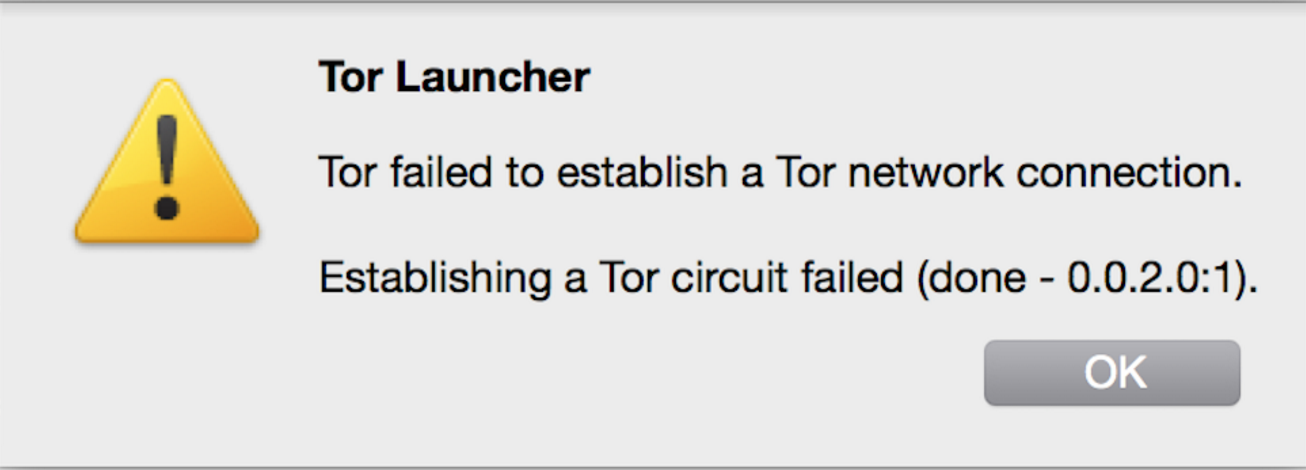
\includegraphics[width=0.5\textwidth]{error.png}
    \caption{An example of a technical error message which our participants did not understand.}
\label{fig:error}
\end{figure}

\pquote{P2}{I don't know what any of those means (list of bridges),or what that (proxy) means at all.}
\pquote{P3}{The vocabulary is really challenging, for someone not doing IT work.}
\pquote{P4}{I didn't know why I was getting back `establishing encrypted directory'---what does that mean?}
The text in the interface intended to guide users through the process was not understood by our participants. The text also gave our participants a sense that the process intimidating for people who did not have a technical background. 

\subsubsection{Connect vs. Configure} 
The first task for our participants was to decide between connecting directly to the Tor network or configuring their connection. Text in the interface tells people that connecting directly ``will work in most situations'' and instructs to configure a bridge or proxy if the ``Internet connection is censored or proxied.'' We found that a majority of our participants did not take the time to read the text on the screen and that if they did, the text did not always soundly influence their decision.

Participants across all censorship environments connected directly to the Tor network. When they did, they did so because they were taking the path of least resistance first or intimidated by the configuration process. 
\pquote{P9}{Configure seemed manual, so I clicked connect.}
\pquote{P14}{The words were confusing. I don't really understand computers. I don't know what configure means in this setting. Hmm, is it going to crash? When you see connect, you want to click it because you really want it to connect.}

Bridges are only necessary when Tor relays are censored, but participants are not able to determine when this happens, or what the difference between a blocked website and a blocked relay. Participant 10 and several other participants in the mild censorship environment opted to configure a connection when a direct connection to the Tor network would have worked. 

\pquote{P10}{I was censored, so I picked the configure.}

Users do not make the optimal choice between connect and configure. This leads to discouragement from attempting a failed connection and wasted time spent waiting for feedback, which lessen the chance for a successful connection. 

\subsubsection{Bridge Configuration} 
When a participant chooses to configure their connection, their next step is to determine whether they need to configure a bridge, and to configure one if necessary. Answering yes to ``Does your Internet Service Provider (ISP) block or otherwise censor connections to the Tor Network'' directs to a bridge configuration screen, whereas answering no skips that screen. We observed that multiple participants struggled with the technical language on the screen, and ultimately decided to try process of elimination. Most participants went with the default option to not configure a bridge. 

\pquote{P7}{The bridge screen was the most challenging. It seemed very technical to me. I don't know what a bridge is.}
\pquote{P12}{I decided which options to choose by process of elimination with trial and error.}

On the bridge configuration screen, participants need to choose between configuring a built-in bridge versus a custom bridge. Participants were unsure of the difference between a built-in bridge and a custom bridge and also why one would use a custom bridge. Most chose obfs3 as their transport, because those were the default options on the screen. 

\pquote{P8}{I have no clue what's the difference between flashproxy, fte, etc. I need to know why the built-in ones aren't working. And why do I need a custom bridge if there are options built in?}
\pquote{P7}{Since it (obfs3) said recommended, it helped actually, and I selected it because it was chosen. I saw the custom bridges option, but I didn't know what to enter there so I went with this (obfs3).}

Participants in E3, the most advanced censorship environment, were required to select a meek bridge (not the default) or to configure a custom bridge. After the first pluggable transport failed and even if the participants deduced that the source of the failed connection was a mis-configured bridge, the pluggable transport names only confused participants and caused odd behaviors. Participants chose transports at random, in order of the list starting from the default, in order of the list starting from the top, choosing familiar-sounding transports first (i.e. meek-amazon over fte), and choosing technical-sounding transports first (i.e. fte over meek-amazon). 

\pquote{P4}{When I saw obfs3 as the recommended option, the next option logically for me was obfs4.}
\pquote{P5}{I tried the pluggable transport that used google, because I noticed that google was working (when I was using a non-Tor browser).}

Users are not qualified to choose transports in an educated order. When our participants chose incorrectly, they spent time testing their wrong hypothesis and got discouraged with each wrong decision. Our participants were resilient and tried for 40 minutes, but we believe that this is a byproduct of the experimental setting and compensation.

\subsubsection{Proxy Configuration} 
After the bridge configuration, the participant is asked if they need a proxy and if so, to configure one. This question also was too technical for most participants.

\pquote{P11}{I think you can only answer this question (does this computer need a local proxy) if you know what a local proxy is. Otherwise, you have no chance.}

For our participants, trying to unsuccessfully configure a proxy was the only mistake that resulted in failure. On the first attempt at configuration, most chose to not configure a proxy. Since the interface passively re-displayed a proxy-related window after an attempted connection regardless of the error, participants incorrectly assumed that they needed a proxy. Participants did not check their incorrect assumption~\cite{wason1960failure}. All who chose to configure a proxy were unsuccessful. 

\pquote{P15}{I didn't know if this computer had any proxy information. I wasn't able to find it if it did.}

None of our censorship environments required our participants to configure a proxy for a successful connection. Participants followed the directions to look at the Internet settings, but they never found the (nonexistent) information.

\subsubsection{Progress Bar} 
Users were generally displeased with the lack of feedback on the progress bar. Users do tolerate delays if they are for security reasons, but only if they understand the reason~\cite{egelmanplease}. Participants in our study usually did not understand the security reason, and experienced delays up to 2 minutes, even in the ideal case in which a user chose the correct configuration on the first attempt. If users chose particular wrong configurations (i.e. a syntactically valid but nonfunctional proxy), they would be waiting for an indefinite period of time. 

\pquote{P16}{There doesn't seem to be a timeout on any of this stuff. Am I waiting long enough? It should work immediately.}
\pquote{P6}{How long does this actually take (to connect)? This took way too long, and I didn't know how long it should take.}
\pquote{P1}{It was hard to figure out if the progress bar wasn't moving because the connection was censored, or if it was just slow.}

Additionally, the progress bar remains empty on subsequent attempts to connect to the Tor Network until the percent progress supersedes the last displayed progress value (i.e. a participant who saw 30\% progress on their first attempt would see 0\% progress in the progress bar until subsequent attempts got at least 40\% progress). The negative feedback of a 0\% progress bar would cause users to assume that their subsequent attempts were wrong, even if they were correct. 

\section{Redesigning the Configuration Interface}
\label{redesign} 
 \begin{figure*}[t]
	\centering
		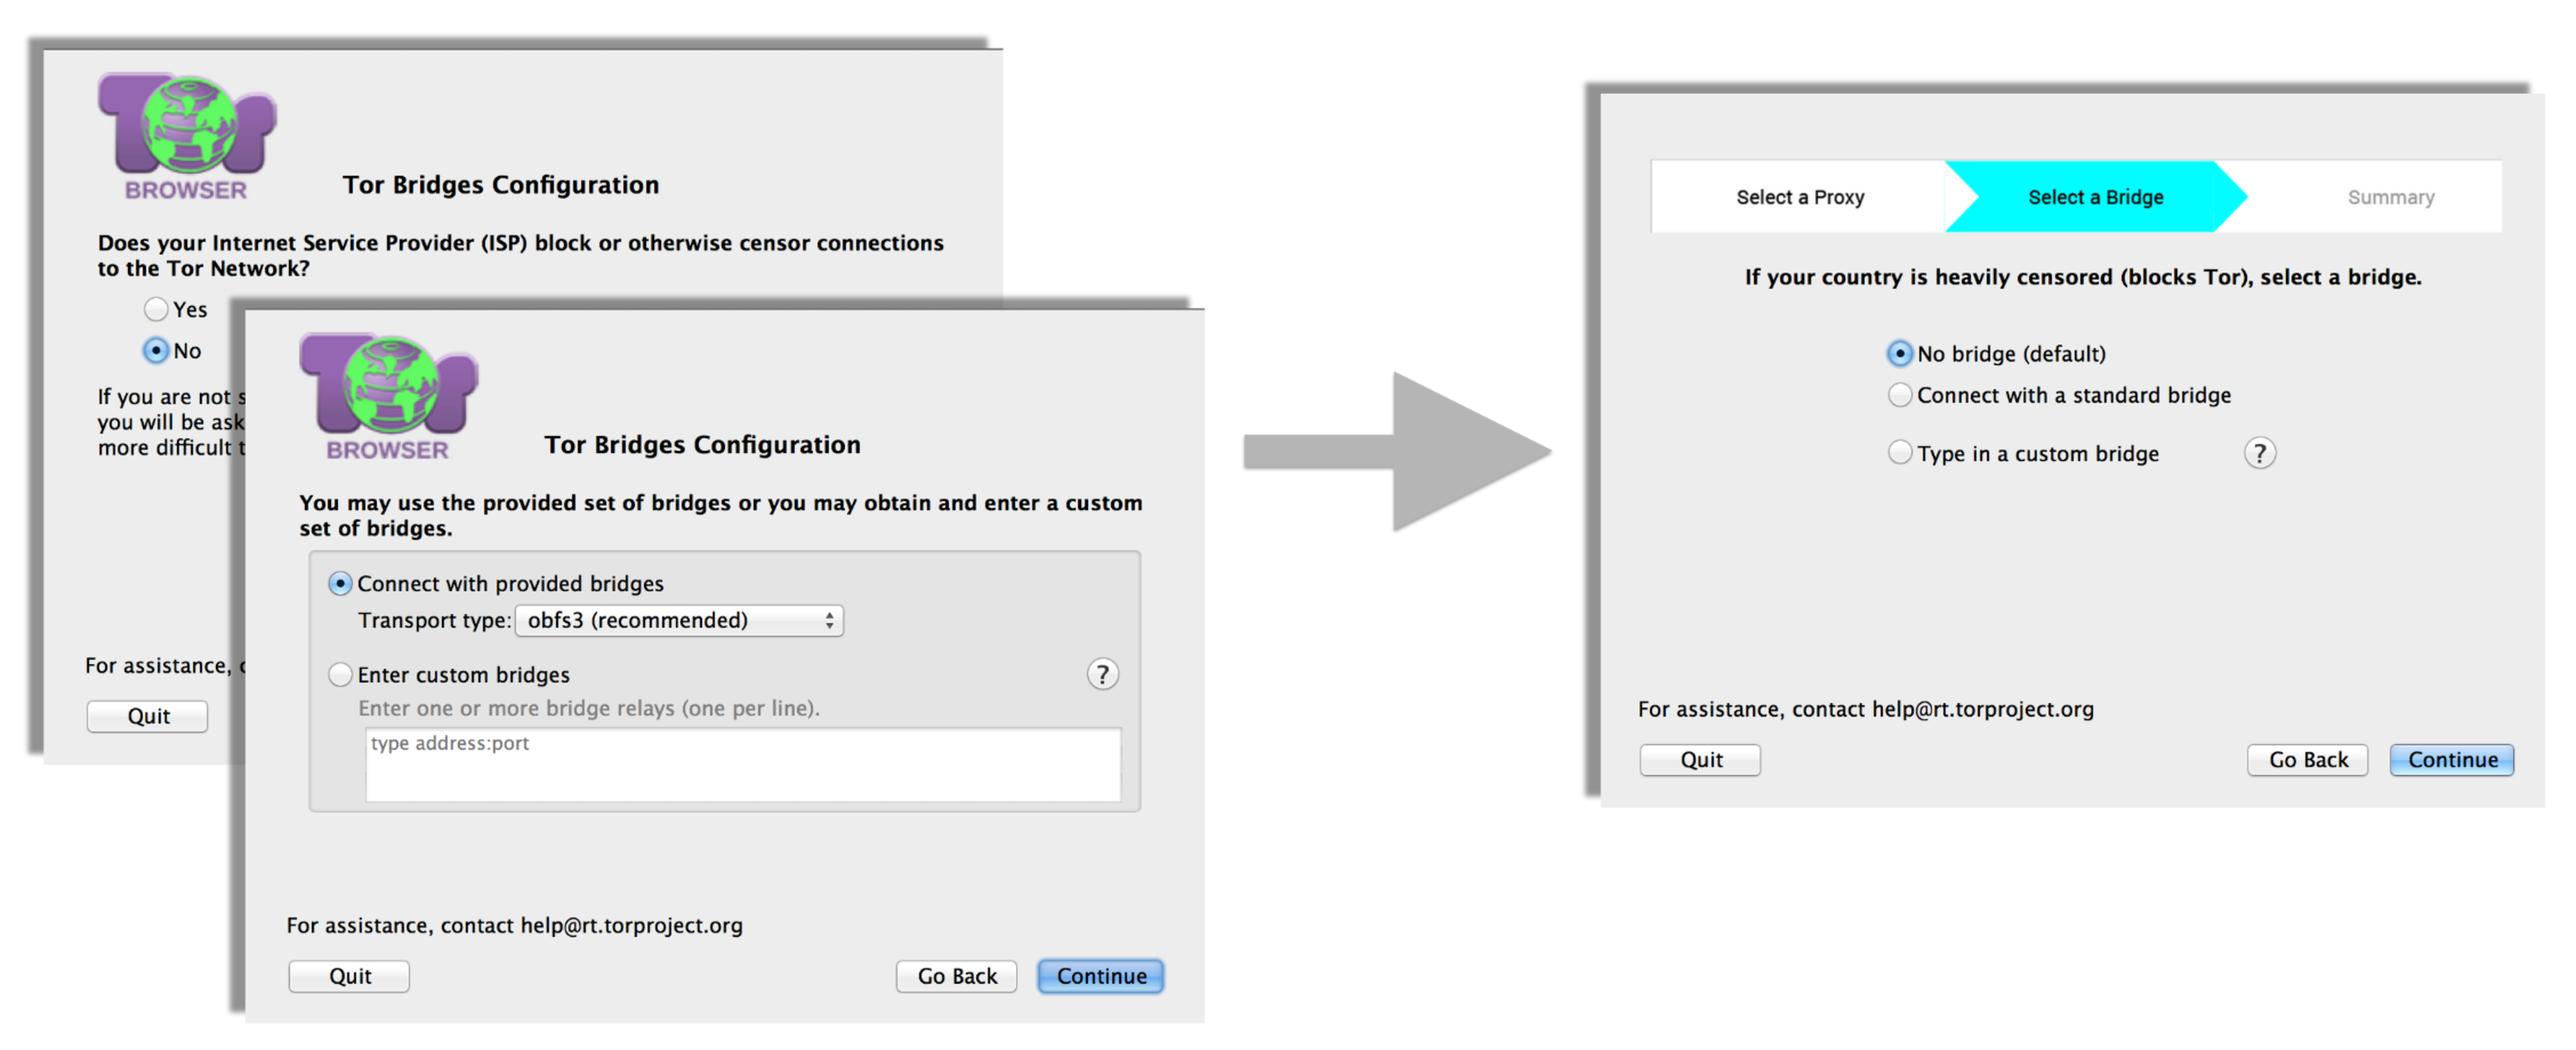
\includegraphics[width=.8\textwidth]{bridge-screens.pdf} 
		\caption{In the ``OLD'' interface, users are asked, ``Does your Internet Service Provide (ISP) block or 
		otherwise censor connections to the Tor Network?'' (B1). A ``Yes'' determines that a bridge should 
		be configured and directs to the bridge configuration screen (B2). 
		The ``NEW'' interface gives users advice on configuring bridges
		while giving the option of not configuring a bridge, on one screen (B).} 
\end{figure*} 

\begin{figure*}[t]
	\centering
		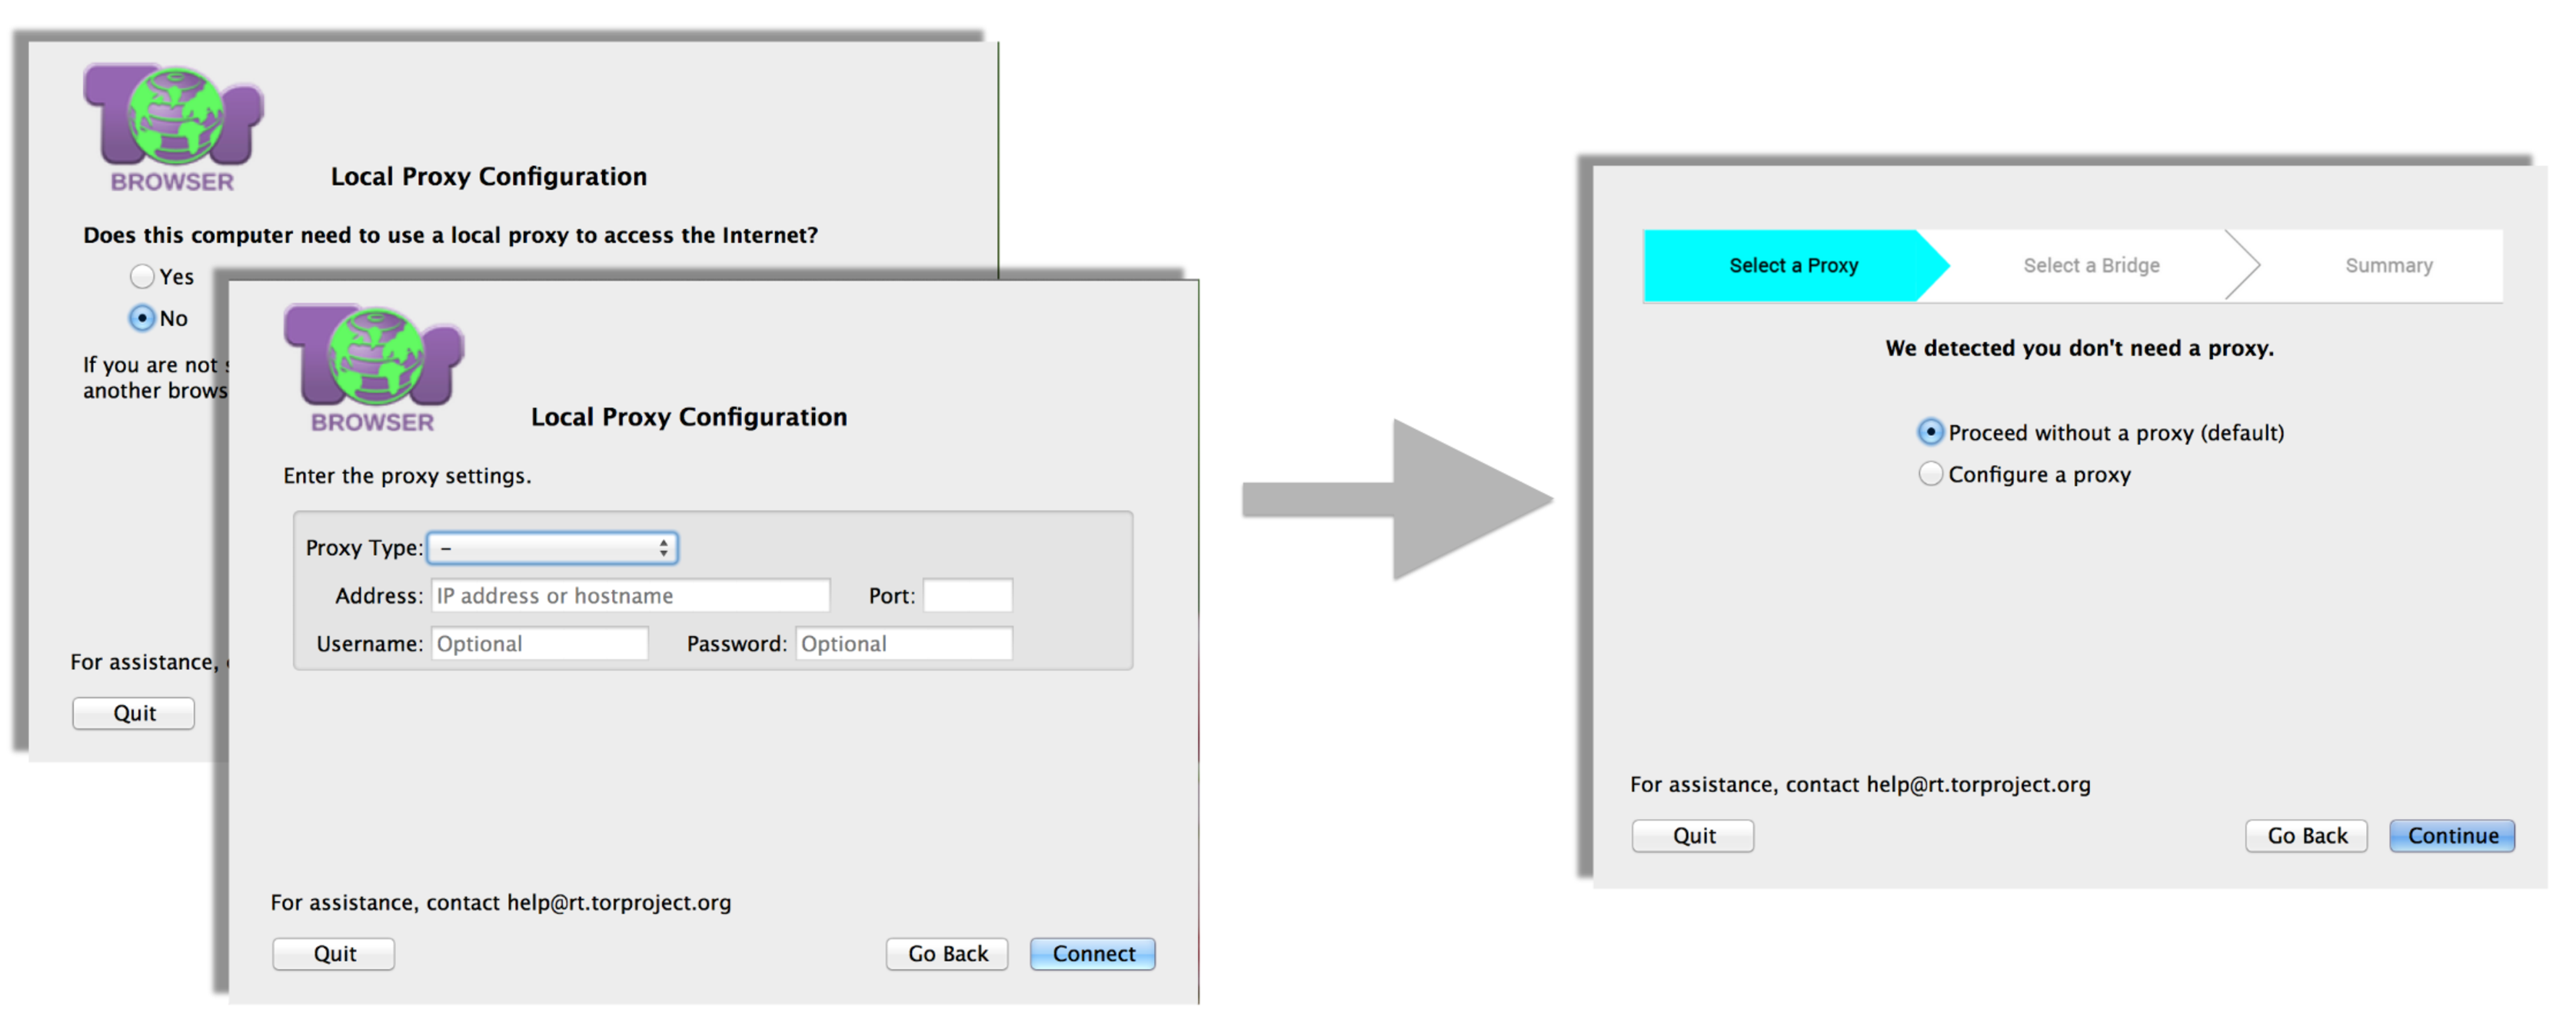
\includegraphics[width=.8\textwidth]{proxy-screens.pdf} 
		\caption{In the ``OLD'' interface, users are asked, ``Does this computer need a local proxy to connect
		to the Internet?'' (P1). A ``Yes'' determines that a proxy should be configured and directs to the 
		proxy configuration screen (P2). The ``NEW'' interface checks the local machine's proxy settings,
		and informs the user whether a proxy is required, and if so, what those settings are (P).}
\end{figure*}

Tor Browser 5.0.3. configuration interface does not adequately meet our heuristic evaluation criteria from Section~\ref{sec:goals}: visibility of system status, user control and freedom, error management, understandable language, and minimal design. We rate the severity of the issue by its frequency, impact, and persistence~\cite{nielsen1994heuristic}:\\

\begin{itemize}
\item {\bfseries Major Problem}: Error messages do not express errors in plain language nor offer solutions. 
\item {\bfseries Major Problem}: The text was too technical for an average user to understand. 
\item {\bfseries Minor Problem}: The configuration is not visible to the users before they connect or while they are connecting.
\item {\bfseries Cosmetic Problem}: The interface can be simplified visually. 
 \end{itemize} 
 
 \label{redesign}
\begin{figure*}[t]
\centering
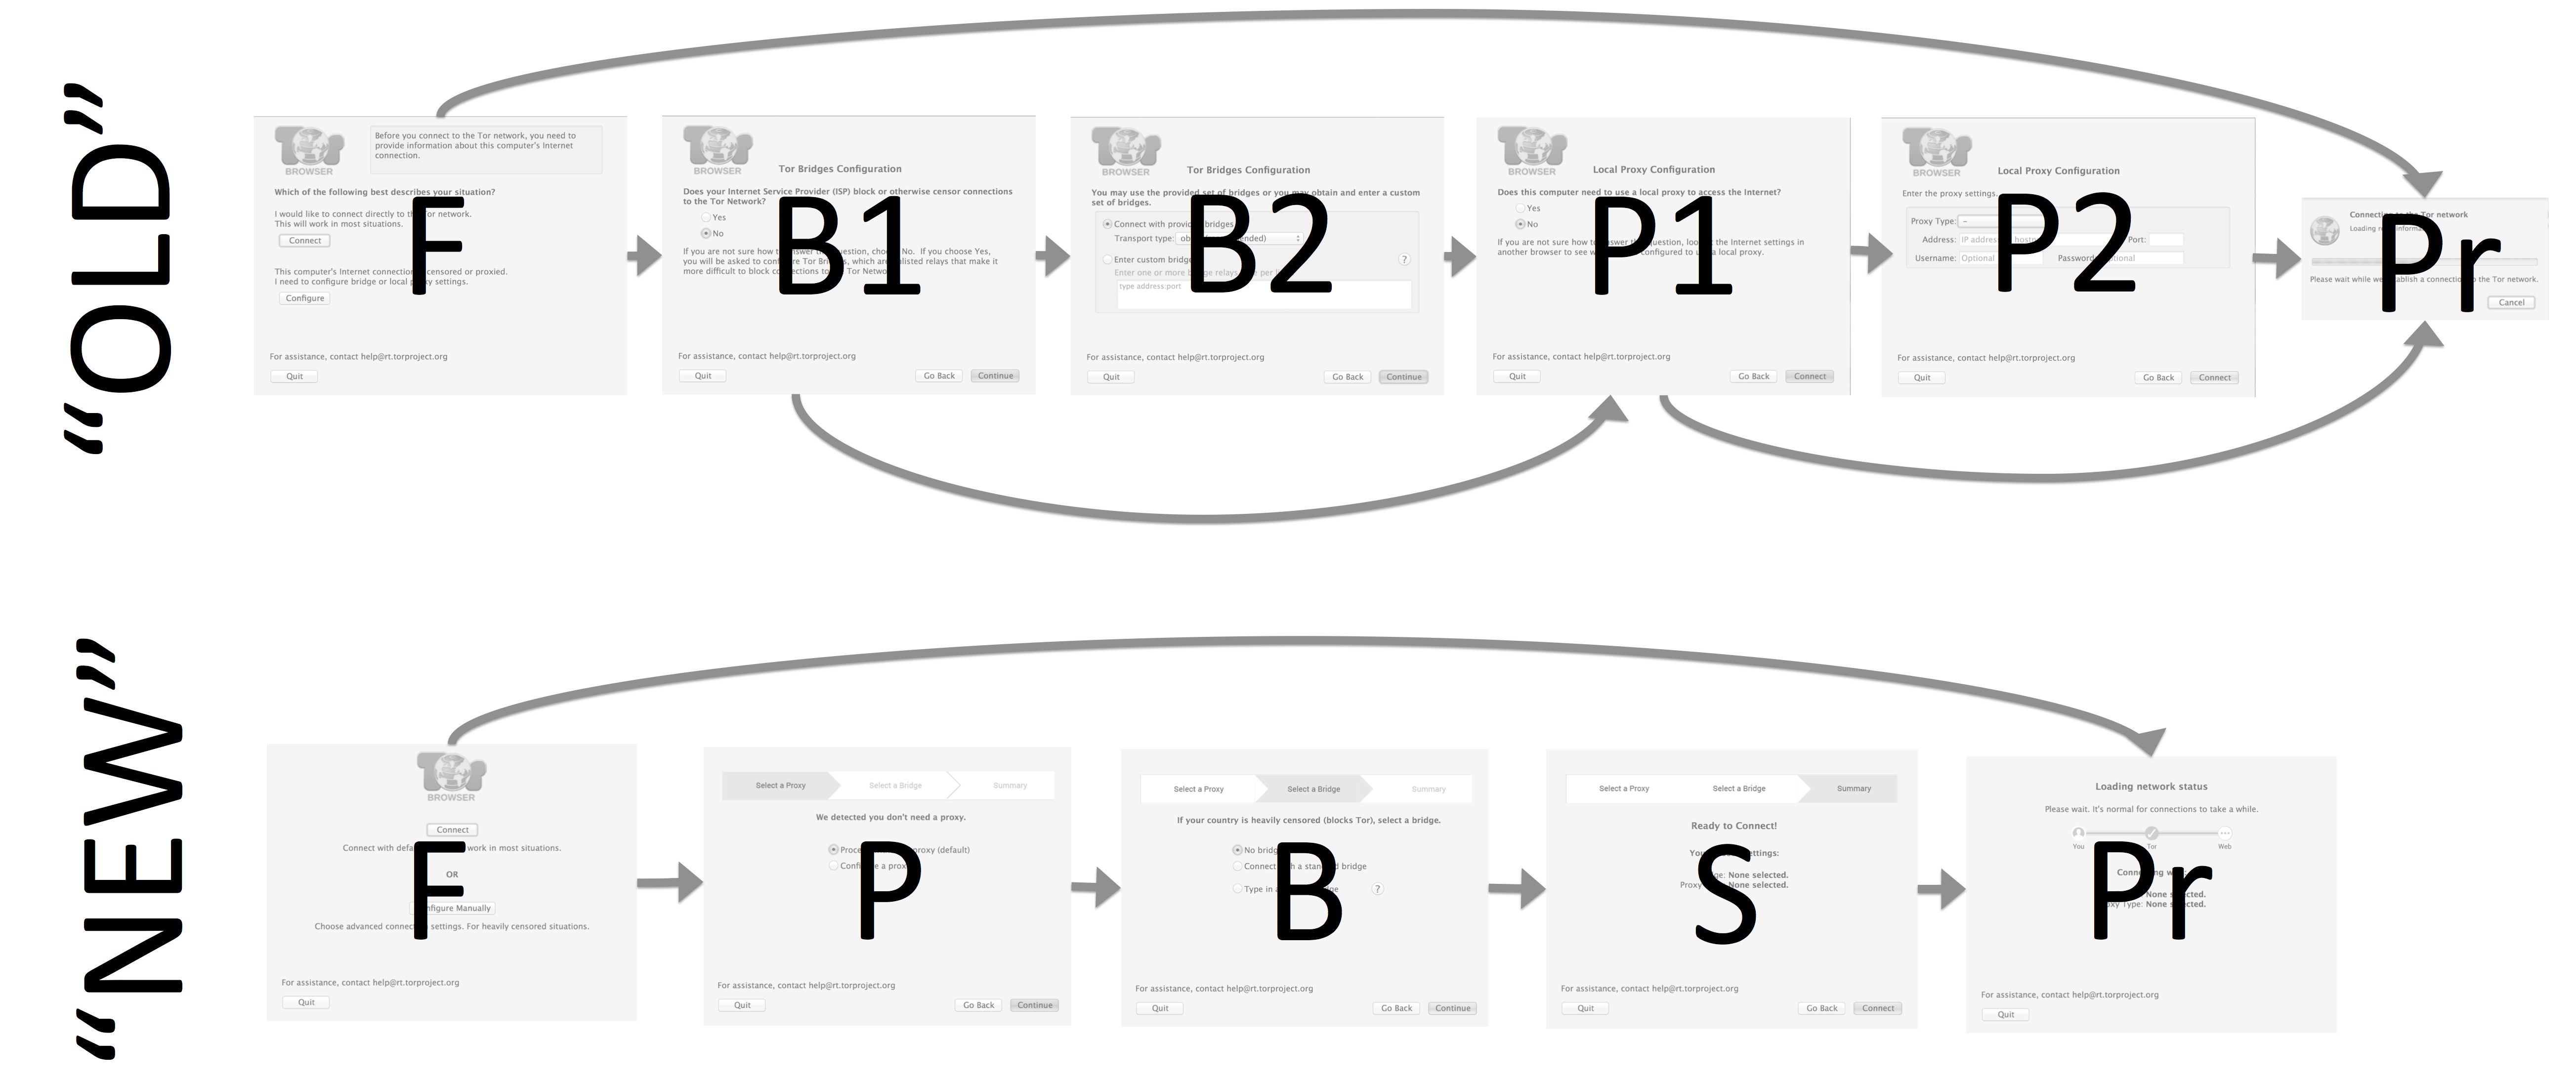
\includegraphics[width=.85\textwidth]{old-and-new-flows.png}
\caption{
Comparison of user flow in the ``OLD'' and ``NEW'' interfaces.
We collapsed the two bridge screens into one 
and also collapsed the two proxy screens into one.
We swapped the order of the bridge and proxy configuration
so it matches the order of network components (compare with Fig.~\ref{fig:topology}).
We added a summary screen as a last step before initiating a connection.\\
\textbf{F}: first screen;
\textbf{B/B1/B2}: bridge screens;
\textbf{P/P1/P2}: proxy screens;
\textbf{S}: summary screen;
\textbf{Pr}: progress bar.
}
\label{fig:flow}
\end{figure*} 

To fix the aforementioned problems, we made the following changes: \\

\begin{enumerate}
\item {\bfseries Added instructions on what to try next on errors.} When an error occurs, text advice on what to try next is shown to the user. Such advice includes trying the connection again, choosing a different bridge, or trying a connection without a proxy. 
\item {\bfseries Reduced overall amount of text and made text less technical.} We make the text more task-centric by focusing on instructing users through the configuration process. Since users generally couldn't understand the technical concepts enough to influence their decisions, giving direct guidance may be a better option. 
\item {\bfseries Added system status visibility.} Before any attempt to connect to the Tor network, a summary screen displays if a bridge or proxy is configured, and if so, what the configurations are. The progress screen also displays the configurations while the connection attempt is being made. 
\item {\bfseries Reduced visual clutter.} We showed options on an as-needed basis and we minimized the amount of text on the screen. For instance, additional fields were hidden until the relevant options were chosen. Additional stylistic simplifications were made, such as removing grouping boxes. 
\end{enumerate} 

Other changes improve empirical goals from Section~\ref{sec:goals}: task completion, time to completion, and safe for high-risk users. 5-6 improve task completion, 7-8 reduce time to completion, and 9-10 builds users' mental models of censorship circumvention and network components involved. Users' full control of the configuration process remains preserved.\\ 

\begin{enumerate}
\setcounter{enumi}{4}
\item {\bfseries Added guidance on choosing connect vs configure.} We labeled the configure option as advanced, manual, and only for heavily censored situations. 
\item {\bfseries Added explicit advice on choosing bridge transports.} The default bridge is still obfs3. There is added text that advises users to try a meek bridge if obfs3 does not work. 

\item {\bfseries Eliminated technical questions.}  We removed questions that determined whether a bridge and proxy should be configured, which were highly technical and challenging for users to answer. There are two fewer screens in the interface.
\item {\bfseries Added auto-detect for proxies.} Auto-detection of proxies can be done locally, by scanning system files. This is safe even for at-risk users, and greatly simplifies the configuration process. 

\item {\bfseries Switched ordering to configure proxies first.} To build users' mental models, network components are configured in a topologically sequential order. Previously, proxies were put after bridge configuration because only a small fraction of users require proxies. With auto-detection, configuring a proxy before a bridge will not burden the users. 
\item {\bfseries Added clear feedback to the progress bar.} We switched the continuous progress bar to a discrete checkpoint based progress bar that shows network components involved in connecting to the Tor network. This aligns with the mental model we are trying to build. As connections are made with components, the progress bar displays a green check, giving immediate feedback to the user. For instance, a user can can now see that the bridge was configured correctly, and they just need to wait to connect to the Tor network. Upon failure, users can see which components have succeeded and which have failed.
\end{enumerate}

The redesigned interface conservatively interacts with users by automating only safe configuration processes and still allowing users to have control over configuring all interacting network components. The design requires more maintenance because of the explicit advice given on which order to select bridges and advice on error messages, which may change as the censorship environments change. 

\section{Quantitative Analyses of the Interfaces (Study 2)}
\label{sec:quantitative}
We performed quantitative research to quantify the existing problems
and the impact of our redesign. Specifically, we collected all events, transitions, 
and state for Tor Browser 5.0.3 and the redesigned Tor Browser.

\subsection{Setup}
We simulated the same three censorship environments from 
our qualitative user study. Details of the E1, E2, and E3
censorship environments and what configurations are necessary for a 
successful connection can be found in Section~\ref{sec:environments}.

We instrumented Tor Launcher 5.0.3 and our redesigned Tor Launcher.
The instrumentation logs recorded every meaningful interaction with the interface---every
button press, every menu selection, every screen change---along with a timestamp.
The logs enabled us to calculate statistics such as the success rate
for each condition. We also recorded the participants' computer screens 
throughout the experiment to capture non-interface activity such as 
web searching and inspection of system networking settings.

We ran our experiment at Xlab, the Experimental Social Science Laboratory at University of 
California, Berkeley. The Xlab allows researchers to run experiments on 36 participants at a time.
There are 36 Windows machines in rows of 4, which are separated by cubicle walls. 
We provided the scripts to set up the simulated censorship environment, install necessary software, 
start the video recording, and save the logs and videos. Our experiment was not limited by Xlab
requirements. However, the configuration interface relies on OS-provided features but testing 
was only done on Windows machines, as a byproduct of using Xlab. 

\subsection{Recruitment}
We recruited about 20 users for each censorship environment
and interface combination, resulting in a total of 124 users. 
Data analysis considerations deem 20 participants in each 
6 interface version and simulated censorship combination a 
minimum to be able to assume normal distributions and 60 participants
testing each interface is large enough to have adequate effect size.

We recruited half of our users from Craigslist, and half of our participants from 
the Xlab participant pool. Although Xlab participants are not limited to UC Berkeley students and staff,
a majority of the participants are from campus. For this reason, we chose to recruit 
half of our participants from Craigslist to ensure a diverse set of participants. 
The recruitment text can be found in Appendix~\ref{quantitative-recruitment}. 

Out of our 124 participants, 59 were recruited from the Xlab pool and the other 65 were
recruited from Craigslist. Ages ranged from 18 to 68
(mu = 28.9, sigma = 12). 56.8\% were male and 
84.8\% of our participants had at least a college education.

\subsection{Procedure}
The one-hour, multi-participant procedure begins when all participants are sitting at their
respective computers in Xlab. Each computer is equipped with an old or modified version
of Tor Browser, Chrome, Firefox, Internet Explorer,  Chrome, and VLC (for screen recording).
Each computer was assigned one of the 6 conditions in the beginning of the study. Participants
were assigned to the seats at random, effectively being assigned a configuration launcher and
simulated censorship environment combination at random. 

Participants are firstly informed of the risks of the study and consenting to data collection.  At
this time, participants are given the chance to leave the laboratory if they do not consent to 
the experiment conditions. When every participant left in the room has turned in their consent
form, the experiment formally begins. A researcher informs the participants that they are in a
simulated censorship environment, where some websites and services are blocked. 
For the full script of what participants have heard, see Appendix~\ref{quantitative-script}. We
instruct them to visit a sample blocked website on a non-Tor browser of their choice to illustrate 
the situation.

After illustrating the censorship environment, participants are asked to 
complete a worksheet that asks to visit one blocked website. 
To mirror the qualitative study, we chose Wikipedia's featured article of the day 
as the blocked website. 

After instructions, researchers maintained minimal interactions with the participants, 
only answering logistical questions. Participants had
about 40 minutes to complete their worksheet.
(In our analysis we defined the cutoff time to be 40 minutes and 8~seconds
in order to include a participant who finished at the wire.)
The participants do not know the details of their censorship environment,
only that they are actively being censored. Participants needed to configure Tor Browser to 
circumvent the simulated censorship. 

After users completed the browsing tasks, they took a short exit survey (Appendix~\ref{quantitative-exit-survey})
collecting their demographics. All users were instructed to sit until the end of the experiment,
regardless of when they had completed their task. After the 40 minutes were up, 
participants were officially informed that their time was up, and were given their payment of 
\$30 for their time. 

\subsection{Results} 
Out of our 124 recruited participants, 116 provided valid data. We have 58 participants who tested the new interface, and 58 who tested the old interface. 38 participants were in E1, 38 participants were in E2, and 40 participants were in E3. Since our experiment ended after 40 minutes, we chose to assign the max time of 40 minutes to participants who did not succeed. Table~\ref{table:participant-summary} summarizes the rate of success and time to success for our participants' based on their interface version and environment combination. 

\begin{table}
\centering
	% Generated by info.R.
	\begin{tabular}{l r r r r}
	& \multicolumn{2}{c}{success rate} & \multicolumn{1}{c}{median time} \\
	& \multicolumn{2}{c}{after 40 minutes} & \multicolumn{1}{c}{to success} \\
	\noalign{\hrule}
	E1-NEW & 19/19 & 100\% & 0:20 \\ % medians of only finished: 0:20 
	E1-OLD & 19/19 & 100\% & 1:01 \\ %medians of only finished: 1:01
	E2-NEW & 18/19 & 95\% & 3:32 \\ %medians of only finished: 3:22
	E2-OLD & 16/19 & 84\% & 5:00 \\ %medians of only finished: 3:13
	E3-NEW & 13/20 & 65\% & 20:56 \\ %medians of only finished: 12:38
	E3-OLD & 10/20 & 50\% & 40:08 \\ %medians of only finished: 18:16 
	\end{tabular}
\caption{
A summary of participants' success in circumventing censorship
given their simulated censorship environment and version of Tor. Those who
failed to connect successfully were assigned the maximum time of 40:08.
}
\label{table:participant-summary}
\end{table}

\subsubsection{Rate of Success} 
5 more participants with the new interface were able to successfully circumvent censorship and connect to the Tor network. Due to the limited number of participants, this difference is not large enough to rule out the possibility of random chance being the cause for the difference. However, this does suggest that users are not less likely to succeed with the new interface based on the changes that were made. 
% impact of version on success: not significant (Mann-Whitney W = 5.5, p-value = 0.8248)
%impact of env on success: not significant (Kruskal-Wallis chi-squared = 4.7059, df = 2, p-value = 0.09509)

Table~\ref{tab:attempts-bridge-proxy} shows the configuration settings of the first successful bootstrap in each environment and interface combination. Note that only four of the default bridges were used to connect successfully for the first time. Users avoid making decisions when a recommendation is given and tend to avoid/fail with more advanced options. Participants who were in environments in that the recommended bridge (obfs3) worked did not configure another bridge, not taking advantage of the various default bridges available to them. Participants who were in environment that required a meek or custom bridge only were able to succeed with a meek-bridge.

\begin{table}
\centering
% Generated by attempts.R, and manually reordered:
\begin{tabular}{r c c c c c c}
& \rotatebox{90}{E1-NEW} & \rotatebox{90}{E1-OLD} & \rotatebox{90}{E2-NEW} & \rotatebox{90}{E2-OLD} & \rotatebox{90}{E3-NEW} & \rotatebox{90}{E3-OLD} \\
no bridge, no proxy & 17 & 13 &  &  &  &  \\
obfs3, no proxy & 2 & 6 & 18 & 16 &  &  \\
meek-amazon, no proxy &  &  &  &  & 7 & 4 \\
meek-google, no proxy &  &  &  &  & 5 & 4 \\
meek-azure, no proxy &  &  &  &  & 1 & 1 \\
no bridge, 3rd-party proxy &  &  &  &  &  & 1 \\
DNF &  &  & 1 & 3 & 7 & 10 \\
\end{tabular}
\caption{
Bridge--proxy combinations that led to the first successful bootstrap
in each environment and interface.
Most E1 participants used a direct connection,
but a few tried a built-in obfs3 bridge.
All the E2 participants who succeeded,
did so with obfs3 (the recommended bridge type)---none tried
a different bridge before obfs3.
All of the successful E3 participants, but one,
used one of the meek bridges.
The remaining E3 participant succeeded in an unexpected way:
by searching the web for an open proxy and configuring it
as the proxy setting.
}
\label{tab:attempts-bridge-proxy}
\end{table}


\subsubsection{Time to Success} 
Although the median times to completion for participants of the new interface are less than those with the old interface (Table~\ref{table:participant-summary}), this difference is not statistically significant. The level of censorship had a significant impact on the time to success. The more difficult the censorship environment, the longer participants took to configure their connection (Kruskal-Wallis chi-squared = 80.926, df = 2, p-value < 2.2e-16). The distribution of participants' time to success can be seen in Figure~\ref{fig:time_to_success_clamped}.
%impact of version on time to success: not significant (W = 1569, p-value = 0.07796)
%impact of env on time to success : significant (Kruskal-Wallis chi-squared = 80.926, df = 2, p-value < 2.2e-16)

\begin{figure}
\centering
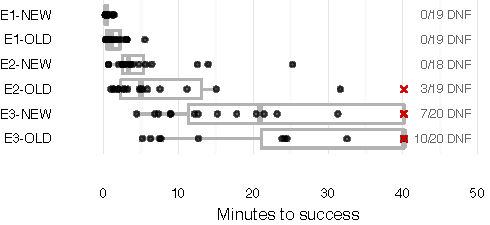
\includegraphics{time_to_success_clamped}
\caption{
Time to first success, by censorship environment and interface.
The dots show the raw completion times,
while the boxplots show the medians and interquartile ranges.
The ``DNF'' figures at the right show the number of participants 
who did not finish in the time allotted.
Here, non-finishing participants are assigned the maximum time of 40:08
for the purpose of computing the median.
}
\label{fig:time_to_success_clamped}
\end{figure}

In our experiment, participants had 40 minutes to circumvent censorship. Figure~\ref{fig:time_to_success_ecdf} shows the cumulative success rates over time. Participants were less and less likely to succeed as time went on. Users in the wild will likely not be motivated to configure their connection for 40 minutes. Table~\ref{table:less_time} shows that if users were only willing to put in a minute or so of their time, users in intermediate and heavily censored environments will be unable to connect. Even if users were willing to dedicate 10 minutes to configuring their connection, most users in heavily censored environments will be unable to connect. Ideally, users should be able to connect to Tor within a couple of minutes, regardless of their censorship environment. We propose ideas on how to achieve this in section~\ref{recommendations}. 

\begin{figure}
\centering
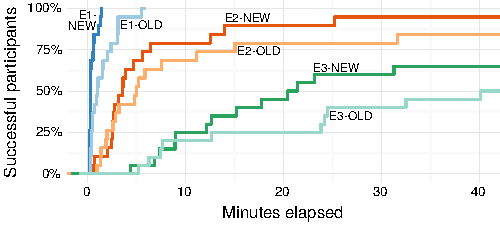
\includegraphics{time_to_success_ecdf}
\caption{
Cumulative success rates over time, by censorship environment and interface.
We stopped participants after 40 minutes. Here, those who did not finish were assigned
an arbitrarily high number greater than 40 minutes for the purposes of plotting. 
}
\label{fig:time_to_success_ecdf}
\end{figure}

\begin{table}
\centering 
	% Generated by info.R:
	\begin{tabular}{l r r r r}
	& \multicolumn{1}{c}{1.5~m} & \multicolumn{1}{c}{10~m} & \multicolumn{1}{c}{20~m} & \multicolumn{1}{c}{40~m} \\
	\noalign{\hrule}
	E1-NEW & 100\% & 100\% & 100\% & 100\% \\
	E1-OLD & 58\% & 100\% & 100\% & 100\% \\
	E2-NEW & 11\% & 79\% & 89\% & 95\% \\
	E2-OLD & 16\% & 68\% & 79\% & 84\% \\
	E3-NEW & 0\% & 25\% & 45\% & 65\% \\
	E3-OLD & 0\% & 20\% & 25\% & 50\% \\
	\end{tabular}
\caption{This Table shows what the success rate would have been
at different cutoff times.
For example, every E1-NEW participant finished within 90 seconds,
but only 58\% of E1-OLD had finished by that time.
After 10 minutes, 79\% of E2-NEW and 68\% of E2-OLD had finished.
After 20 minutes, 45\% of E3-NEW and only 25\% of E3-OLD had finished.}
\label{table:less_time}
\end{table}

\subsubsection{Additional information} 
We summarize each participant's actions throughout the experiment in Figure~\ref{fig:all-participant-edges}. Each row in Figure~\ref{fig:all-participant-edges} corresponds to a participant in our experiment. The bar represents a participants' path through the interface, illustrating time spent on each screen, transitions between screens, how many attempts were made, and if they were eventually successful. 

\begin{figure*}
\centering
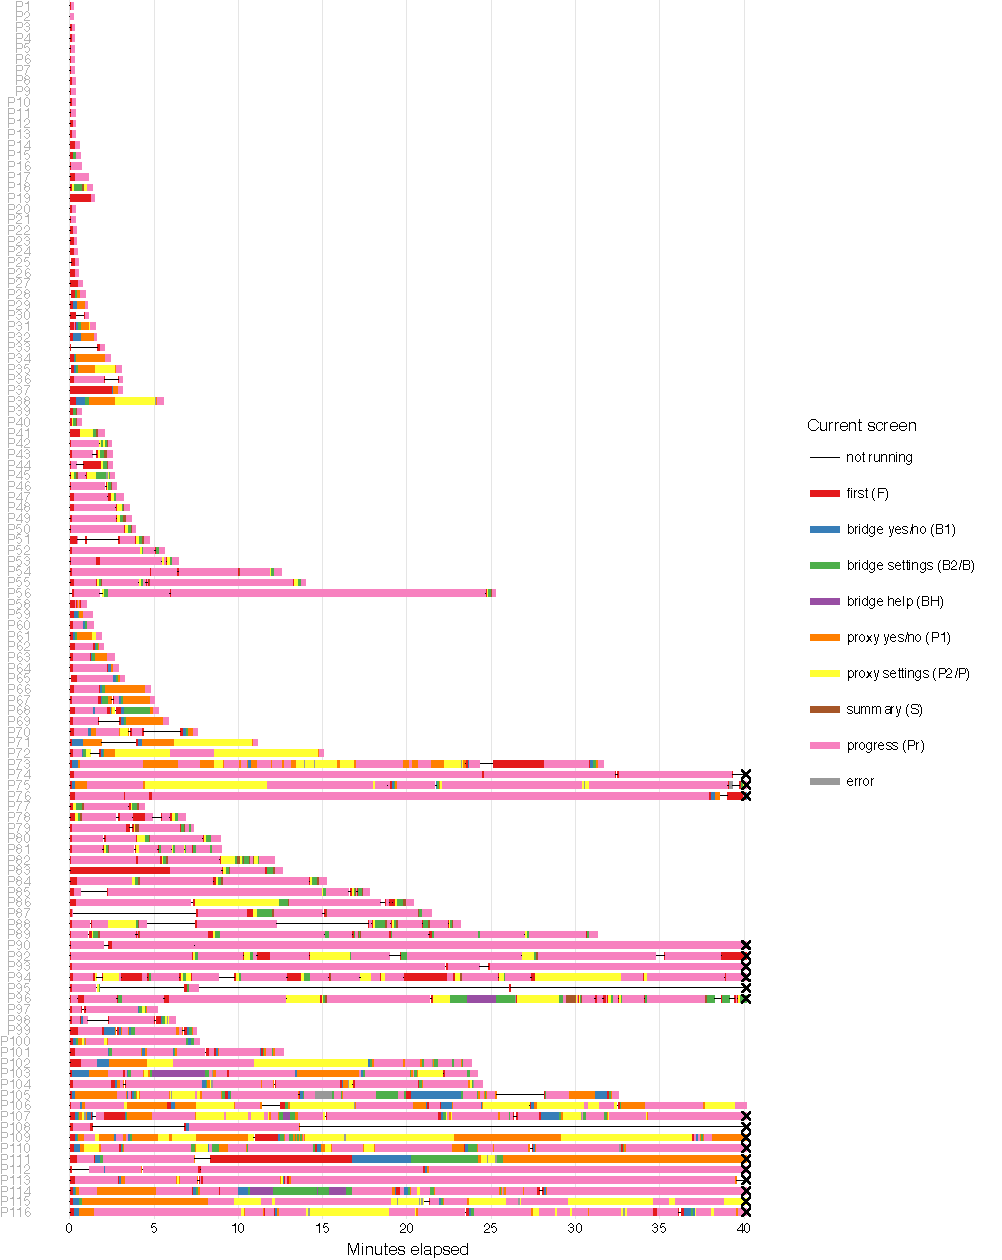
\includegraphics{all-participant-edges}
\caption{
Summary of participants' actions throughout the entire experiment.
Different colors indicate which screen was shown at each moment.
The narrow black lines show the times when the configuration interface
was not running; i.e., a participant was doing something else
such as searching the web in another browser.
The overall length of the lines show the total time to completion,
except for those we cut off after approximately 40 minutes.
}
\label{fig:all-participant-edges}
\end{figure*}

While we did not find a statistically significant difference between the overall time to success between the old and new versions of the interface, the time to success was largely dominated by the time spent waiting to connect to Tor, rather than actively configuring the interface. Table ~\ref{table:overall_time} shows the time spent on each screen while participants used the interface, which shows that participants spent 57\% of their overall time at the progress screen. Participants using the new interface and old interface waited spent approximately the same amount of time overall on the progress screen (359 minutes versus 339 minutes), which accounts for 78\% and 45\% of their overall time, respectively. We attribute this to a combination of instructions that tell the user to ``wait a couple minutes'' because connections usually take a while to bootstrap and the lack of timeout on the progress screen which keeps the users waiting indefinitely, which were present in both versions of the interface. 

\begin{table}
\centering
	\begin{tabular}{c r r r r r}
	 & First & Proxy & Bridge & Summary & Progress \\
	\noalign{\hrule}
	All &  10\% & 24\% & 8\% & 1\% & 57\% \\
	NEW & 9\% & 7\% & 4\% & 2\% &  78\% \\
	OLD & 10\% & 35\% & 11\% & 0\% & 45\% \\
	E1 & 33\% & 16\% & 23\% & 1\% & 27\% \\
	E2 & 11\% & 18\% & 8\% & 1\% & 63\% \\
	E3 & 8\% & 27\% & 8\% & 1\% & 57\% \\
	\end{tabular}
\caption{overall time} 
\label{table:overall_time}
\end{table}

Perhaps a more meaningful measurement of time is the amount of times participants actively spent configuring their connection. We define this as the amount of time that participants spent on the interface, except for time spent on the progress screen. This is a simplified notion active configuration time, since some participants searched for help on the web while they were waiting. However, this behavior was equally likely in the new and old interface conditions.

The new interface results a statistically significant reduction in the overall active configuration time (Mann-Whitney Z = -3.055, p-value = 0.00225, effect size = 0.284), while maintaining the same probability for success for the user. We believe that getting rid of the technical bridge and proxy questions, instructing participants that they did not need a proxy, and simplifying the interface attributed to the reduction in time. 
%The impact of the environment on active time is significant (Kruskal-Wallis chi-squared = 51.978, df = 2, p-value = 5.166e-12)

\subsection{Discussion} 
This section talks about general trends in user behavior, common failure cases, and our recommendations for 
improving the Tor configuration interface. 

\subsubsection{Observations}
These are general observations made from our data set of participants, which may have biases.\\

\begin{description}
%connect vs configure
\item {\bfseries Users try the easy path first.}
81\% (94 of 116) of first attempts were to connect directly, 86\% (50 of 116) from the new interface and 76\% (44 of 116) from the old interface. 

% impacts of making the proxy page ``automated'' 
\item {\bfseries Users wasted time configuring proxies.} Overall, 57\% of participants' active configuration time was spent on the proxy screens. Participants with the new interface spent 31\% of their active time configuring proxies and participants in the old interface spent 63\%.

% impacts of giving people advice on which transport to choose.
\item {\bfseries Certain transports were chosen with high probability.}
Of those who tried an obfs3 bridge and failed, 
66\% (10 of 15) participants with the new interface and 38\% (5 of 13) participants with the old interface chose meek as their second bridge. Flashproxy was also a popular choice. Many bridges were never chosen. 

%error messages
\item {\bfseries There were (almost) no error messages.} Many waited for minutes at the progress screen, but never saw an error message. Only one participant ever saw an error message. We are unable to state the efficacy of our attempts to make error messages more understandable and instructive for lack of data.  

% progress bar
\item {\bfseries People waited a long, long time at the progress bar.}
From observing videos, participants genuinely wait, dutifully following the directions.   
\end{description} 

It is unclear why users with the new interface chose to configure proxies after explicitly being told that they do not need one, if they chose meek bridges based on our advice, and why they chose to wait longer at the progress screen. 

\subsubsection{Reasons for Failure} 
Failure is common. 64\% (74 of 116) of first attempts to connect failed and 79\% (376 of 462) of total attempts to connect failed. Although most participants eventually succeeded, 20\% (23 of 116) failed entirely. Reasons for failure were determined by a combination of log processing (i.e. how much time was spent on a particular screen) and video observation (i.e. observing what they searched for online while they were stuck). \\ 

\begin{description}
\item {\bfseries Only connected directly. (8/23)} These participants tried a direct connection. When that failed, they tried the same configuration, over and over, without trying other configurations, no matter how many times they failed. It was common to restart the interface, check Internet settings, and wait between subsequent attempts. 
\item {\bfseries Didn't know what to do next. (6/23)} After a failed direct connection and a failed default obfs3 bridge connection, these participants did not know what to do next. They often tried those configurations again or gave up. 
\item {\bfseries Thought that they needed a proxy (6/23)} After a couple failed attempts, these participants assumed that they needed a proxy. They spent the time trying to configure a proxy, usually without trying other bridges. 
\item {\bfseries Used the bridges auto-responder incorrectly (3/23)} Three participants in our heavy censorship environment figured that the recommended bridge and most hard-coded bridges were not working and found the auto-responder through the help button. However, they all failed to get a response. For details, see Appendix~\ref{failed-participants}.
\end{description} 

Some participants chose to download their own version of Tor. We discarded these participants' data and do not count this behavior as a failures or success. While some downloaded their own version without trying the provided one on their desktop, others did so after feeling frustrated with the provided version. For unfortunate details of where participants downloaded tor when torproject.org was blocked, see Appendix~\ref{tor-downloads}.

\subsubsection{Recommendations}
\label{recommendations}
Based on our observations of general behavioral trends and common failure cases, we make the following recommendations to increase success rate and decrease overall time spent in the interface: \\

\begin{description}
\item {\bfseries Automate configuration after failure.} After one unsuccessful attempt, the user has already indicated to their censor that they are connecting to Tor. Automating the configuration process thereafter will have no increase in risk, bu can help a majority of users. 64\% of participants who failed their first attempt. Users in more difficult censorship environments are more likely to benefit from this, as 5\% of participants in the mild censorship environment , 84\% participants in intermediate censorship environment, and 100\% of participants in the heavy censorship environment failed the first time.
\item{\bfseries Hide infrequently used options.} Informing users that they did not need a proxy was not enough to deter users from spending time on configuring a proxy. Only a small fraction of the Internet population requires a proxy to connect to the Internet. Hiding the proxy screen by default and only showing it after it has been detected as necessary can focus user efforts on configuring bridges.
\item {\bfseries Be explicit about recommendations.} Being explicit about the order in which a user should choose bridges will result in higher rates of success and lessen cognitive load on the user. Most participants followed recommendations about which bridge to choose, and many did not know what to do after the recommended bridge failed. 
\item{\bfseries Set a timeout on the progress bar.} Informing users that they have failed earlier will decrease the overall time to success, create an opportunity to give suggestions, and reduce user frustration. 
\item{\bfseries Have a user-tolerant auto-responder.} Having the auto-responder default respond with bridges or catching common errors (such as typing ``get bridges'' in the subject line) can help those who need custom bridges. 
\end{description} 

We believe that these changes have can greatly help future users connect to the Tor network. We also encourage best practices, such as providing a summary screen to let the user know the configuration settings before connecting, having a checklist progress bar to give users feedback on what network component needs configuring, and rewriting screen text and error messages to be more instructive and understandable. 

\section{Limitations} 
The interface was only tested on Windows machines, which were the only types of machines in Xlab. The configuration interface uses the native operating system's elements and their respective styling, so an interface looks slightly different across different operating systems. Participants who are not accustomed to using Windows machines may have been slower than usual to complete the given task, but this effect should affect all of our conditions equally. 

Our study was conducted in an inorganic setting, which can cause our participants to be under or over-motivated. Our participants had a monetary incentive to connect to Tor, whereas a real user in a censored environment would want to reach a particular website or service. The nature of the experiment places social pressure to attempt connect for the whole duration of the session, whereas participants may have given up earlier if they were not in an organic setting.   

We did not test cases in which the user is required to configure a custom bridge or proxy. Our participants were from one geographic location in the United States and are able to speak English.

\section{Future Work} 
Throughout the qualitative user study, redesign of the interface, and the quantitative user study, we collaborated and communicated with Tor developers. Redesigning the configuration interface was a mutual interest. In fact, Tor version {\color{red} 5.?.?} incorporated textual and navigational changes based on our redesigned interface. We plan to continue our work with Tor developers to integrate changes we found to be helpful. This process will entail debugging our code, merging changes with the current version of Tor, making high-fidelity graphics that align with style guides, and finalizing the advice to give to users in the interface. 

We took an approach that optimized for the average case user yet was conservative enough in automation to allow users to connect without leaking that they use Tor. Additional user studies that focus specifically on users in heavily censored environments, or increasing the amount of automation in the configuration process can yield to higher rates of success and faster time to success. We encourage future work to explore some of the non-conservative changes and alternate approaches that we were not able to test in these series of experiments.\\

\begin{description}
\item{\bfseries Automate the configuration.} This sounds like a radical idea, but this wouldn't harm users today. Additionally, our study finds that most users would leak that they are using Tor when trying to circumvent an advanced censor. 
\item{\bfseries Ask about the risk.} Ask the users if they would be at risk if the process was automated, and automate the configuration process for all who are not at risk. The ones at risk will configure manually. The complication with this approach is that users may not be qualified to answer this question or may not trust Tor to answer honestly. 
\item{\bfseries Ask if users if they know what to do.} We ask users if they know how to configure a bridge and proxy, and automate the configuration process if they do not. However, there are ethical implications of making mistakes on behalf of the users if there is risk involved. 
\end{description}

Ideally, we want users in censorship environments across the world to succeed in connecting to the Tor network in a couple of minutes. We believe that this is possible with continued improvements to the interface. 

%\section {Acknowledgments}
%{\color {red} Rowilma del Castillo for setting up Xlab, Nima Fatemi, Isabela Bagueros, Georg Koppen, and the UX team for giving feedback, and Cecile Basnage for reviewing the UI of circumvention tools.} 
%{\color {red} Tor Browser devs for taking our recommendations to heart and implementing changes.}

\section{Conclusion} 
We conducted a series of experiments to improve the Tor launcher configuration interface, which helps users circumvent censorship using Tor Browser. The qualitative user study interviews a screened 16 participants about their experience trying to circumvent mild, intermediate, and heavy censorship with the current interface, giving insight into common struggles, such as difficulty in answering technical questions, feeling unqualified to make technical choices, and not receiving feedback in the event of a failed configuration. This feedback is used to guide the redesign of the configuration interface. 

We test the impact of our changes on 124 participants in the quantitative user study to find that that the changes made cause a statistically significant reduction in the time participants spent configuring their connection, with no decrease in success rates. We observe and quantify common behavioral trends based on logs and video recordings of our participants, and offer recommendations that we believe will greatly increase the success rate and time to success for future users. 

\bibliographystyle{abbrv}
\nocite{*}
\bibliography{pets2017-paper}

\appendix
\section{Participant Worksheet Text} 
\label{participant-worksheet}
Imagine you live in an oppressive country that censors part of the Internet. We have simulated this in the laboratory by blocking certain websites and services. The purpose of this experiment is to evaluate the use of Tor browser, which is a browser that can circumvent censorship and let you visit blocked websites. For instance, www.torproject.org is blocked. Check this by going to the site on a standard browser, like Firefox, Chrome, or Internet Explorer. It will fail to load, when you can visit other sites.

To complete this worksheet, you will need to set up Tor browser (on your desktop) correctly and use it to get to blocked site. If you can visit wikipedia, then you know that you have successfully circumvented censorship.

\section{Qualitative User Study Recruitment Posting} 
\label{qualitative-recruitment}
We are recruiting participants for an in-person research study at the University of California, Berkeley. You will need to come in to our lab and perform tasks on a computer for an hour or less. You will be compensated \$30 for participating. 
No special knowledge and no technical experience is required. If you are interested, fill out the survey at \textit{<survey link>}. 

\section{Qualitative User Study Prescreening Survey} 
\label{qualitative-prescreening}
We are recruiting participants for an in-person research study at the University of California, Berkeley. You will need to come in to our lab and perform tasks on a computer for an hour or less. You will be compensated \$30 for participating. No special knowledge and no technical experience is required.\\

\begin{enumerate}
\item{Please select when you are available. We will assign you an hour experiment time slot during one of those times.}
\item{I am able to provide my own transportation to the University of California, Berkeley campus.}
\item{Thank you for your interest! Please provide an email address where we can contact you to share more logistical details.}
\item{we are looking for a very small number of participants, so unfortunately, we may not be able to accommodate everyone who applies. Would you like us to let you know about future opportunities?}
\item{What is your gender?}
\item{What is your age?}
\item{Please select your highest completed (or current) level of education.}
\item{What is your occupation?} 
\item{Do you speak any languages other than English fluently?}
\item{If you have a personal computer, what kind do you use?}
\item{Which of the following terms have you heard of? \textit{<answer choices: a checkboxlist of the the following terms: malware, proxy services, phishing, SSL, X.511 certificates, Tor>}}
\item{How often do you use the following software or features? \textit{<answer choices: a grid of radio buttons. Software/features (rows): HTTPS on web pages, proxies or other censorship circumvention tools, virtual private networks (VPN), file or whole-disk encryption, anonymity systems (e.g., Tor), email encryption (e.g., PGP), chat or instant messaging encryption, voice communication encryption. Frequency (columns): never, less than once a month, a few times a month, several times a week, daily.>}}
\end{enumerate}
Thank you for filling out this form. You are now done!

\section{Qualitative User Study Introduction Script} 
\label{qualitative-script} 
Imagine you live in an oppressive country that censors part of the Internet. We have simulated this in the laboratory by blocking certain websites and services.  The purpose of this experiment is to evaluate the use of Tor browser, which is a browser that can circumvent censorship and let you visit blocked websites. Currently, torproject is blocked (you can check this by going to torproject.org on a standard browser, like Firefox, Chrome, or Internet Explorer). 

To circumvent censorship successfully, you will need to set up Tor browser correctly and use it to get to Wikipedia. If you are able to reach the website, then you know that you have successfully circumvented censorship. Fill out the question on the worksheet. This isn't intended to be hard, just write what you see. We want to just check you saw the website. 

Before you start, do you have any questions about what you are asked to do? 

\section{Post-Experiment Standard Interview Questions}
We asked our participants these questions after they were given time to configure Tor Browser. \\

\begin{enumerate}
\item{Can you talk us through what you did along with what you were thinking at the time?}
\item{What was most challenging part of connecting?}
\item{Were there any unfamiliar terms?}
\item{How did you decide which options to choose?}
\item{What did you think about using Tor?}
\item{What is one change you would recommend?} 
\item{Did you need any additional information?} 
\end{enumerate}  

In addition to these questions, we asked our participants about specific questions based on their observation, usually regarding a specific choice in action, a particular screen they seemed stuck on, and any errors they encountered during the configuration process. 

\section{Quantitative User Recruitment Posting}
\label{quantitative-recruitment}
We are recruiting up to 40 participants for a user study at UC Berkeley. The experiment will involve basic Internet browsing tasks. You are not eligible if you have participated in our previous sessions.\\

\indent Payment: \$30 Amazon gift card\\
\indent Duration: 1 hour \\
\indent Where: Xlab at Hearst Memorial Gymnasium\\

\textit{<list of sessions>}\\

To be eligible, you must be an adult (18 or older). This is to comply with university policies on research. 

If you are interested: 1. Email lnl@berkeley.edu with the sessions you are able to attend. We will confirm your participation and assign you a session. 2. Come to Xlab at the appointed time for the experiment.

\section{Quantitative User Study Introduction Script} 
\label{quantitative-script} 
Imagine you live in an oppressive country that censors part of the Internet. We have simulated this in the laboratory by blocking certain websites and services.  The purpose of this experiment is to evaluate the use of Tor browser, which is a browser that can circumvent censorship and let you visit blocked websites. Currently, torproject is blocked (you can check this by going to torproject.org on a standard browser, like Firefox, Chrome, or Internet Explorer). 

To circumvent censorship successfully, you will need to set up Tor browser correctly and use it to get to Wikipedia. Tor is already installed for you. On the desktop, you should see a globe icon that says ``Start Tor Browser.'' If you are able to reach the website, then you know that you have successfully circumvented censorship. Fill out the question on the worksheet. This isn't intended to be hard, just write what you see. We want to just check you saw the website. 

Afterward, we ask you to take a short survey to collect some information about you. The link is also on your worksheet.
We will give you time to complete this task. If you finish early, we ask that you sit at your desk until the remainder of the hour. Since we are recording your screen, we ask that you don't do anything personal afterward, like checking your email.

Before you start, do you have any questions about what you are asked to do? 

\section{Quantitative User Study Exit Survey} 
\label{quantitative-exit-survey}
We'd like to know more about you.  All of your answers will be stored separately from any identifying information in order to protect your confidentiality.

This survey is part of a research project being conducted by the University of California, Berkeley. If you have any questions about your rights or treatment as a research participant in this study, please contact the University of California at Berkeley's Committee for Protection of Human Subjects at 510-642-7461, or email subjects@berkeley.edu. If you agree to participate, please click Next below.\\

\begin{enumerate}
\item{What is your participant ID? (This can be found on the sticker on the left hand corner of the desk you are currently sitting at.)}
\item{What is your gender?}
\item{What is your age?}
\item{Please select your highest completed (or current) level of education}.
\item{What is your current occupation?}  
\end{enumerate}

Thank you for participating in our experiment. You are now done! Please sit at your desk for the remainder of the experiment. Our researchers will formally announce the end of the experiment. 

\section{Failed Participants} 
\label{failed-participants}

Only connected directly (8/23): 
\begin{itemize}
\item E2-NEW-X21-20160323-133257 
\item E2-OLD-X04-20160330-181928
\item E2-OLD-X10-20160331-153028
\item E3-NEW-X05-20160324-132535
\item E3-NEW-X17-20160323-133002
\item E3-OLD-X06-20160328-132053
\item E3-OLD-X06-20160330-161525 
\item E3-OLD-X12-20160330-182011
\end{itemize} 

Didn't know what to do next (6/23): 
\begin{itemize}
\item E3-NEW-X11-20160330-161511
\item E3-NEW-X11-20160331-174655
\item E3-NEW-X23-20160323-133346
\item E3-OLD-X06-20160331-174650
\item E3-OLD-X12-20160331-153055
\item E3-OLD-X30-20160328-134412
\end{itemize} 

Thought that they needed a proxy (6/23): 
\begin{itemize}
\item E2-OLD-X10-20160328-132828
\item E3-NEW-X18-20160330-170145
\item E3-NEW-X17-20160328-160037
\item E3-OLD-X06-20160325-175101
\item E3-OLD-X06-20160330-181926
\item E3-OLD-X24-20160328-155926
\end{itemize} 

Used the bridges auto-responder incorrectly (3/23): 
\begin{itemize}
\item E3-NEW-X23-20160328-155924 (Figure~\ref{autoresponder1})
\item E3-OLD-X12-20160325-140813 (Figure~\ref{autoresponder2})
\item E3-OLD-X24-20160328-133857 (Figure~\ref{autoresponder3})
\end{itemize}   

\begin{figure}[h]
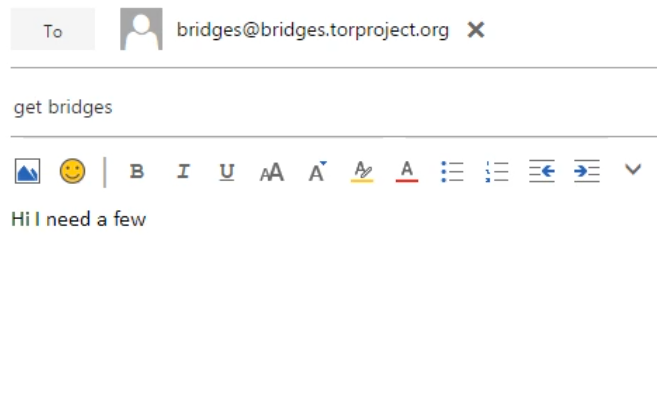
\includegraphics[width=0.5\textwidth]{../experiment/processing/failed-participants/20160325-140813-bridgeresponder-redacted.png}
\caption{The message that E3-NEW-X23-20160328-155924 attempted to send to the bridge auto-responder. The message was sent to the wrong address: bridges@bridges.torproject.org instead of bridges@torproject.org.}
\label{autoresponder1}
\end{figure} 

\begin{figure}[h]
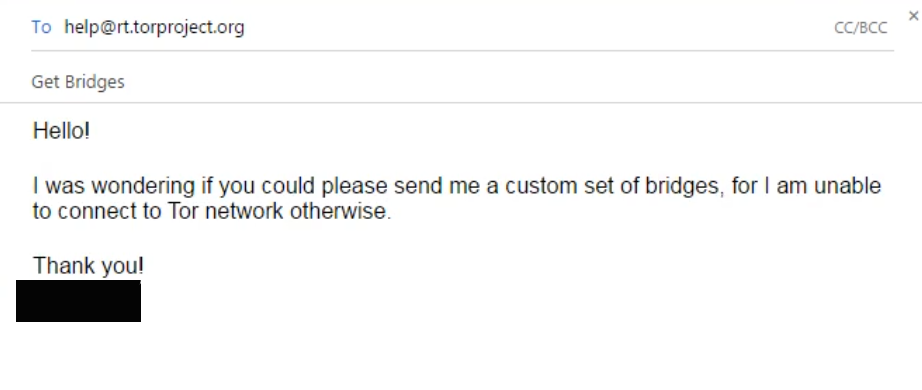
\includegraphics[width=0.5\textwidth]{../experiment/processing/failed-participants/20160328-133857-bridgeresponder-redacted.png}
\caption{The message that E3-OLD-X12-20160325-140813 accidentally sent to the helpdesk rather than the bridge auto-responder. The participant should have used the address bridges@torproject.org, not help@rt.torproject.org. Since the helpdesk address is not an auto-responder, there was no reply.}
\label{autoresponder2}
\end{figure} 

\begin{figure}[h]
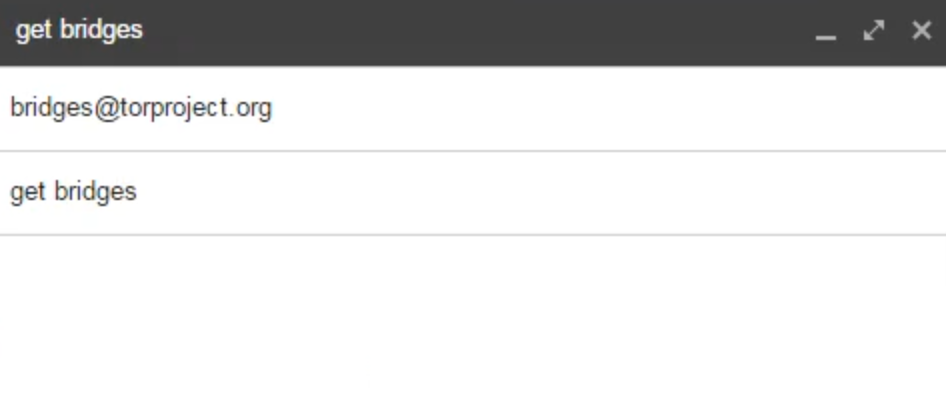
\includegraphics[width=0.5\textwidth]{../experiment/processing/failed-participants/20160328-155924-bridgeresponder.png}
\caption{The message that E3-OLD-X24-20160328-133857 sent to the bridge auto-responder. A correct message is a ``get bridges'' in the body of the message, with any non-empty subject. Since this request was incorrectly formatted, there was no reply.}
\label{autoresponder3}
\end{figure} 

\section{Tor Downloads}
\label{tor-downloads}

Participants that downloaded Tor (5/124): 
\begin{itemize}
\item E1-OLD-X32-20160328-134531(Figure \ref{mirror})
\item E2-NEW-X21-20160323-133257 (Figure \ref{techspot})
\item E2-OLD-X10-20160323-132505 (Figure \ref{downloadio})
\item E2-OLD-X28-20160328-134111 (Figure \ref{driverupdate})
\item E3-NEW-X11-20160330-161511 (Figure \ref{softsonic})
\end{itemize} 

Sources of downloads: 
\begin{itemize}
\item {\bfseries techspot.com -> 1download.io}: the ad firefox yahoo ad result for ``tor browser downloads.'' 
\item {\bfseries driverupdate.net}: the 5th chrome google search result for ``tor browser download.'' 
\item {\bfseries www.torservers.net/mirrors}: the first chrome google search result for ``tor browser mirror.''
\item {\bfseries techspot.com}: the 5th chrome google search result for ``tor browser download.''
\item {\bfseries softsonic.com}: the 2nd firefox yahoo search result for ``tor browser.''
\end{itemize}

\begin{figure}[h]
\label{downloadio}
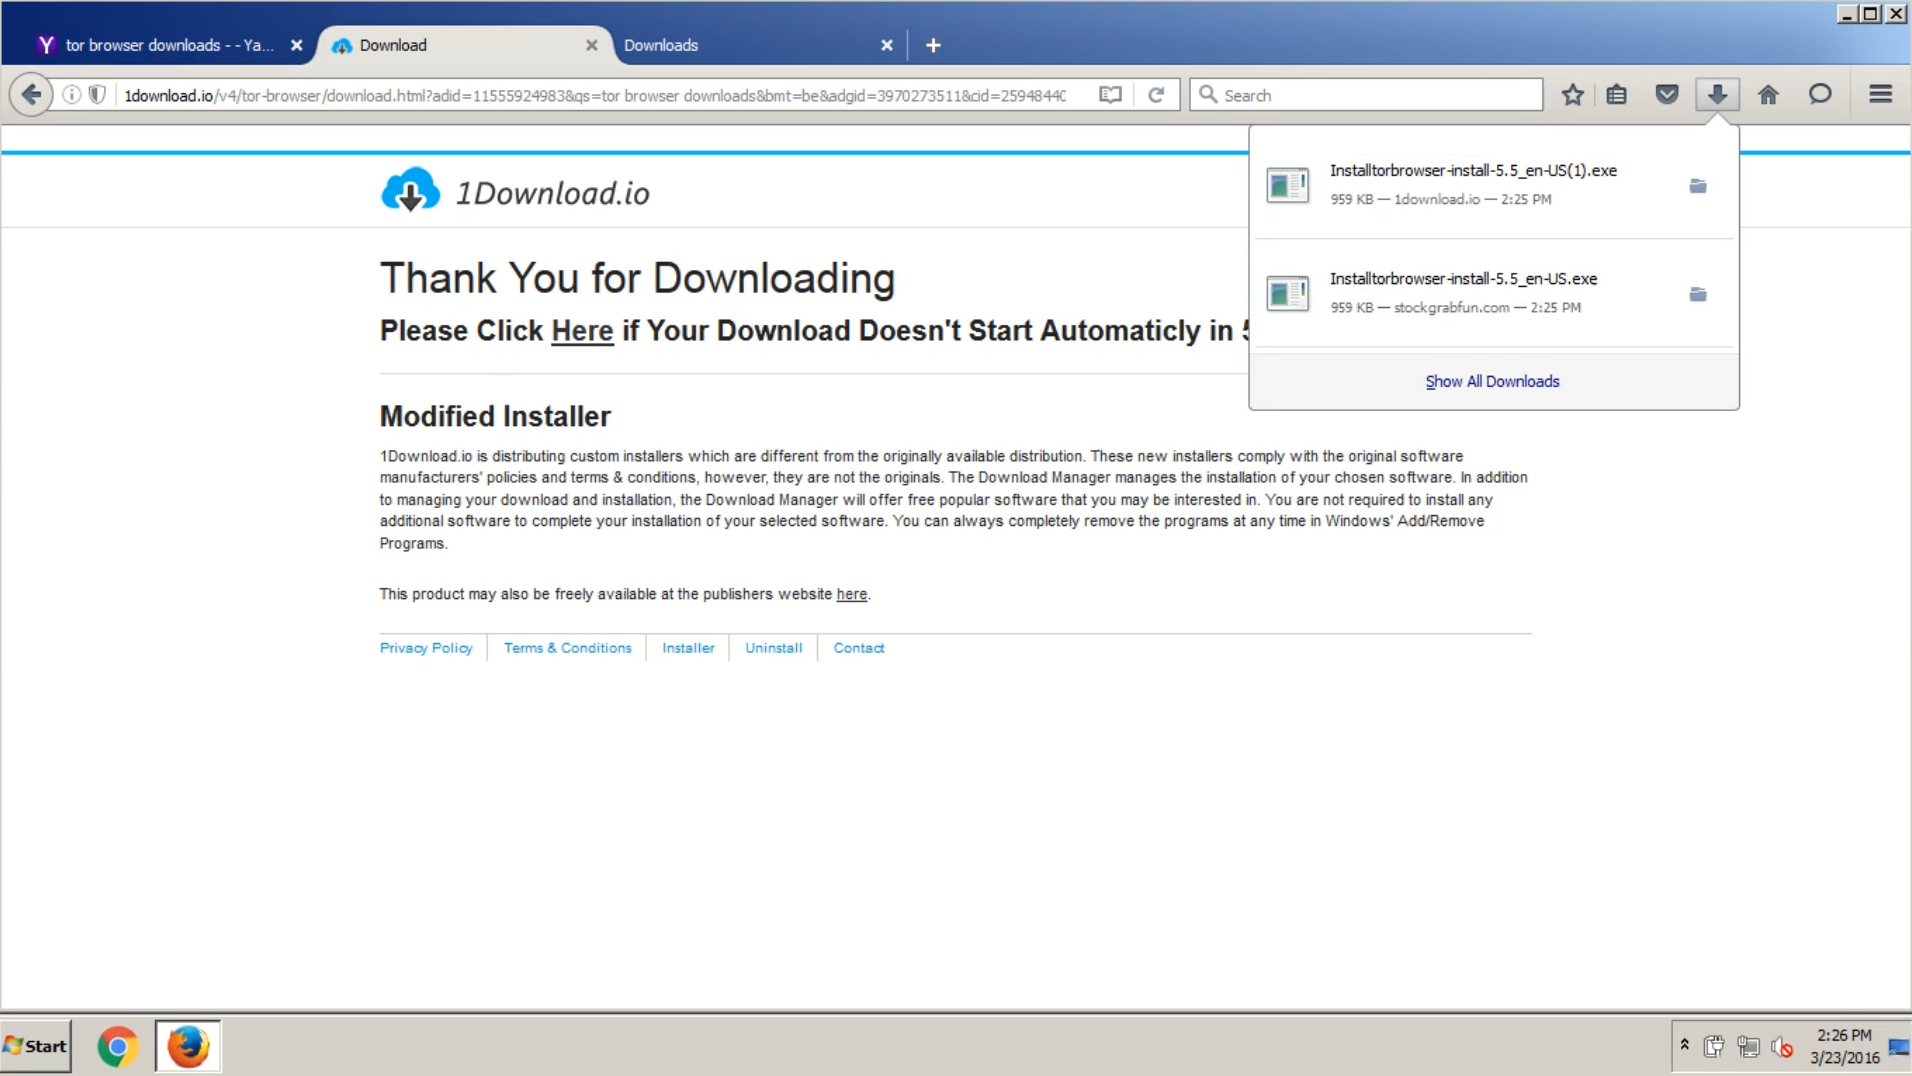
\includegraphics[width=0.5\textwidth]{../experiment/processing/bad-participants/X10-20160323-132505-1downloadio.png}
\caption{X10-20160323-132505 attempted downloaded Tor Browser from TechSpot.com, but clicked on one 
a download link which was not from TechSpot.com. The download was from 1download.io, a suspicious source.}
\end{figure} 

\begin{figure}[h]
\label{driverupdate}
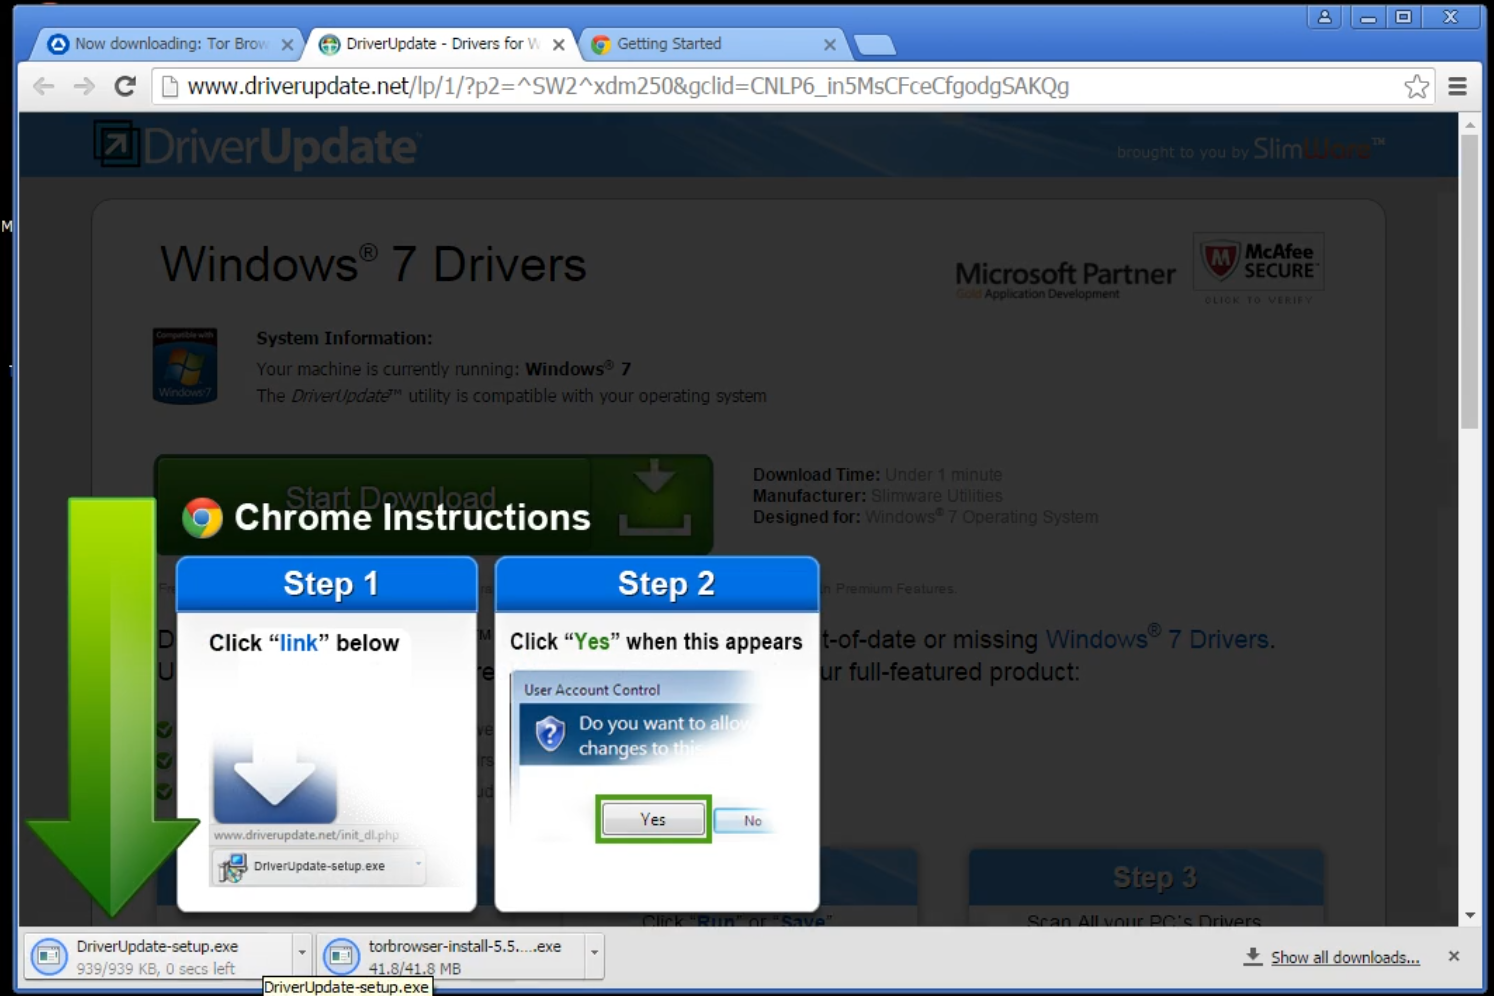
\includegraphics[width=0.5\textwidth]{../experiment/processing/bad-participants/X28-20160328-134111-driverupdate.png}
\caption{X28-20160328-134111 downloaded Tor Browser from DriverUpdate, a suspicious source. Two executables
are downloaded, and the website instructs the user to run an executable named ``DriverUpdate-setup.exe,'' which the
participant dutifully does before running the Tor Browser executable.}
\end{figure} 

\begin{figure}[h]
\label{mirror}
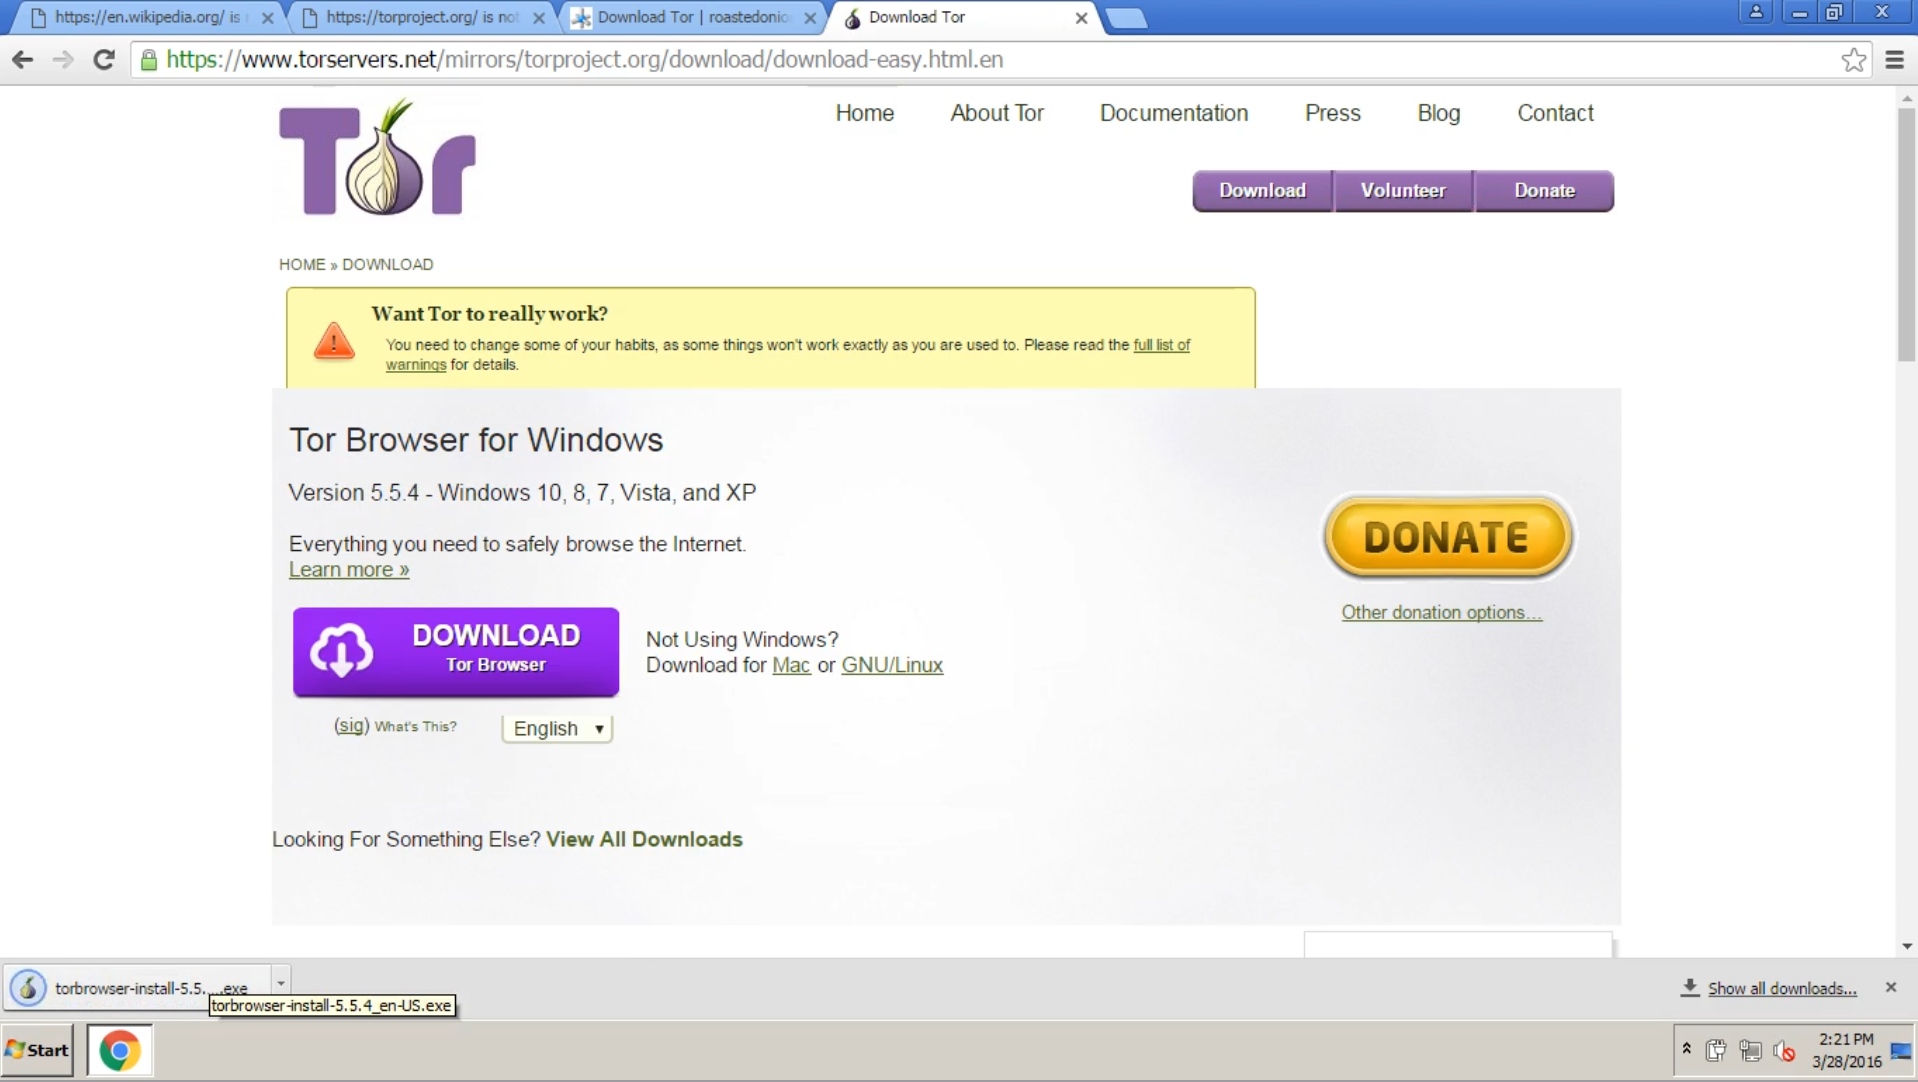
\includegraphics[width=0.5\textwidth]{../experiment/processing/bad-participants/X32-20160328-134531-mirror.png}
\caption{X32-20160328-134531 downloaded Tor Browser from a legitimate Tor Browser mirror,www.torservers.net/mirrors.}
\end{figure}

\begin{figure}[h]
\label{techspot}
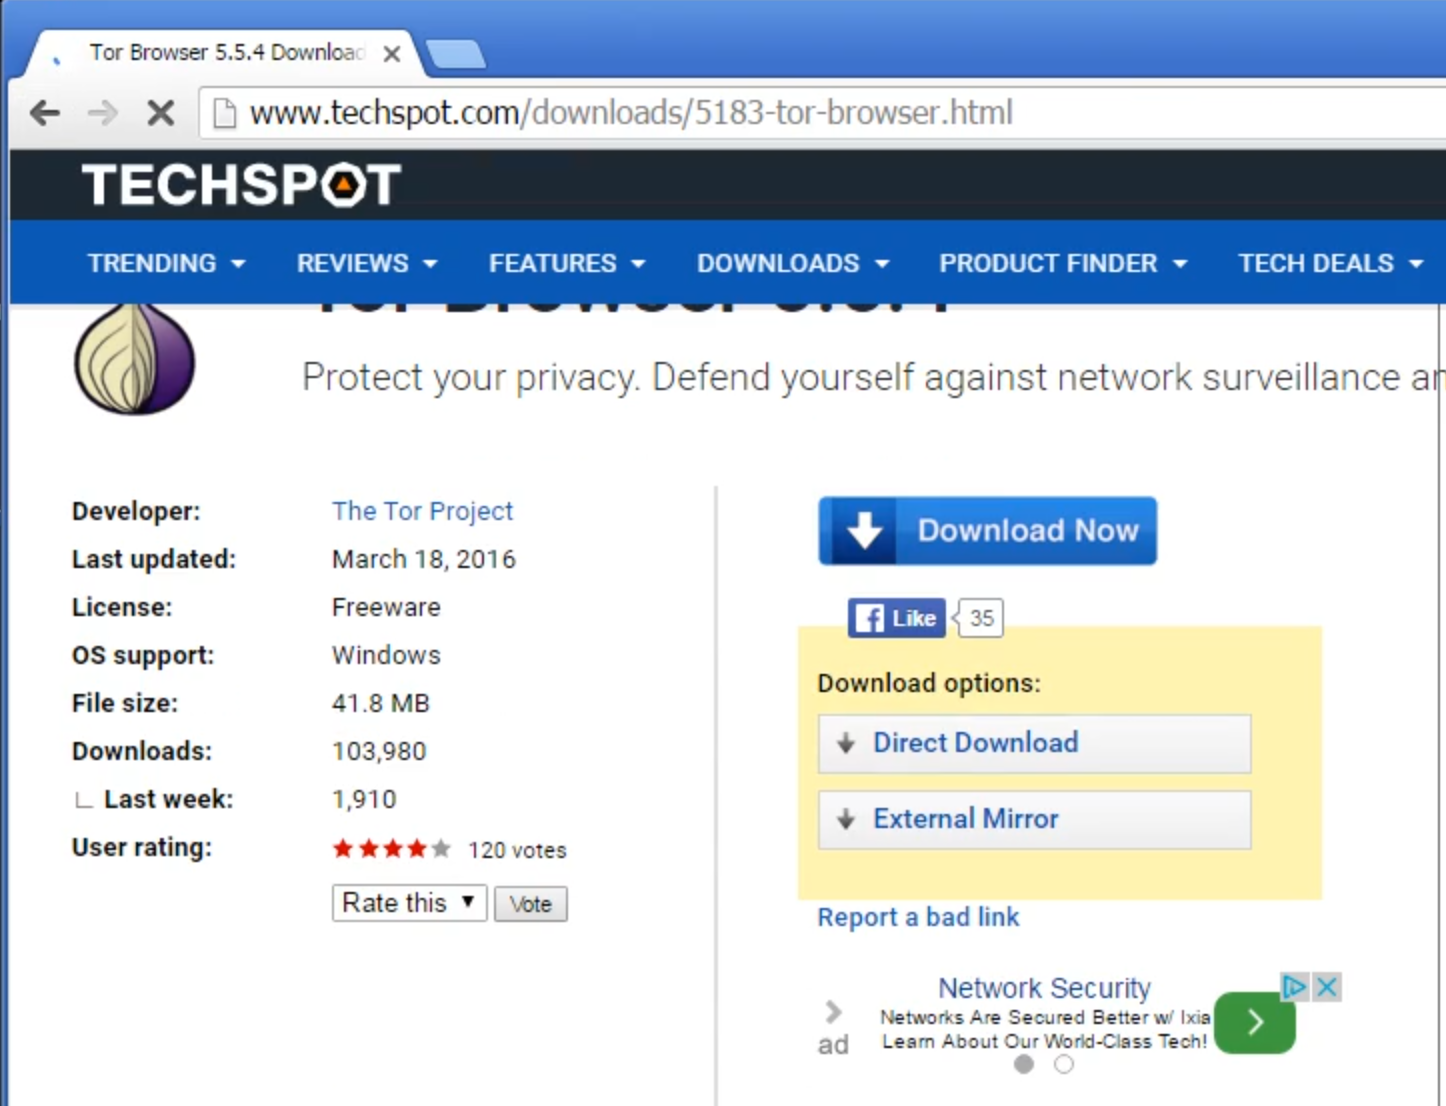
\includegraphics[width=0.5\textwidth]{../experiment/processing/bad-participants/20160323-133257-techspot.png}
\caption{E2-NEW-X21-20160323-133257 downloaded Tor Browser from TechSpot, clicking on the download link from 
TechSpot (the white ``Direct Download'' button). X10-20160323-132505 in Figure \ref{downloadio} clicked the blue ``Download Now'' button and downloaded from a different source.}
\end{figure}

\begin{figure}[h]
\label{softsonic}
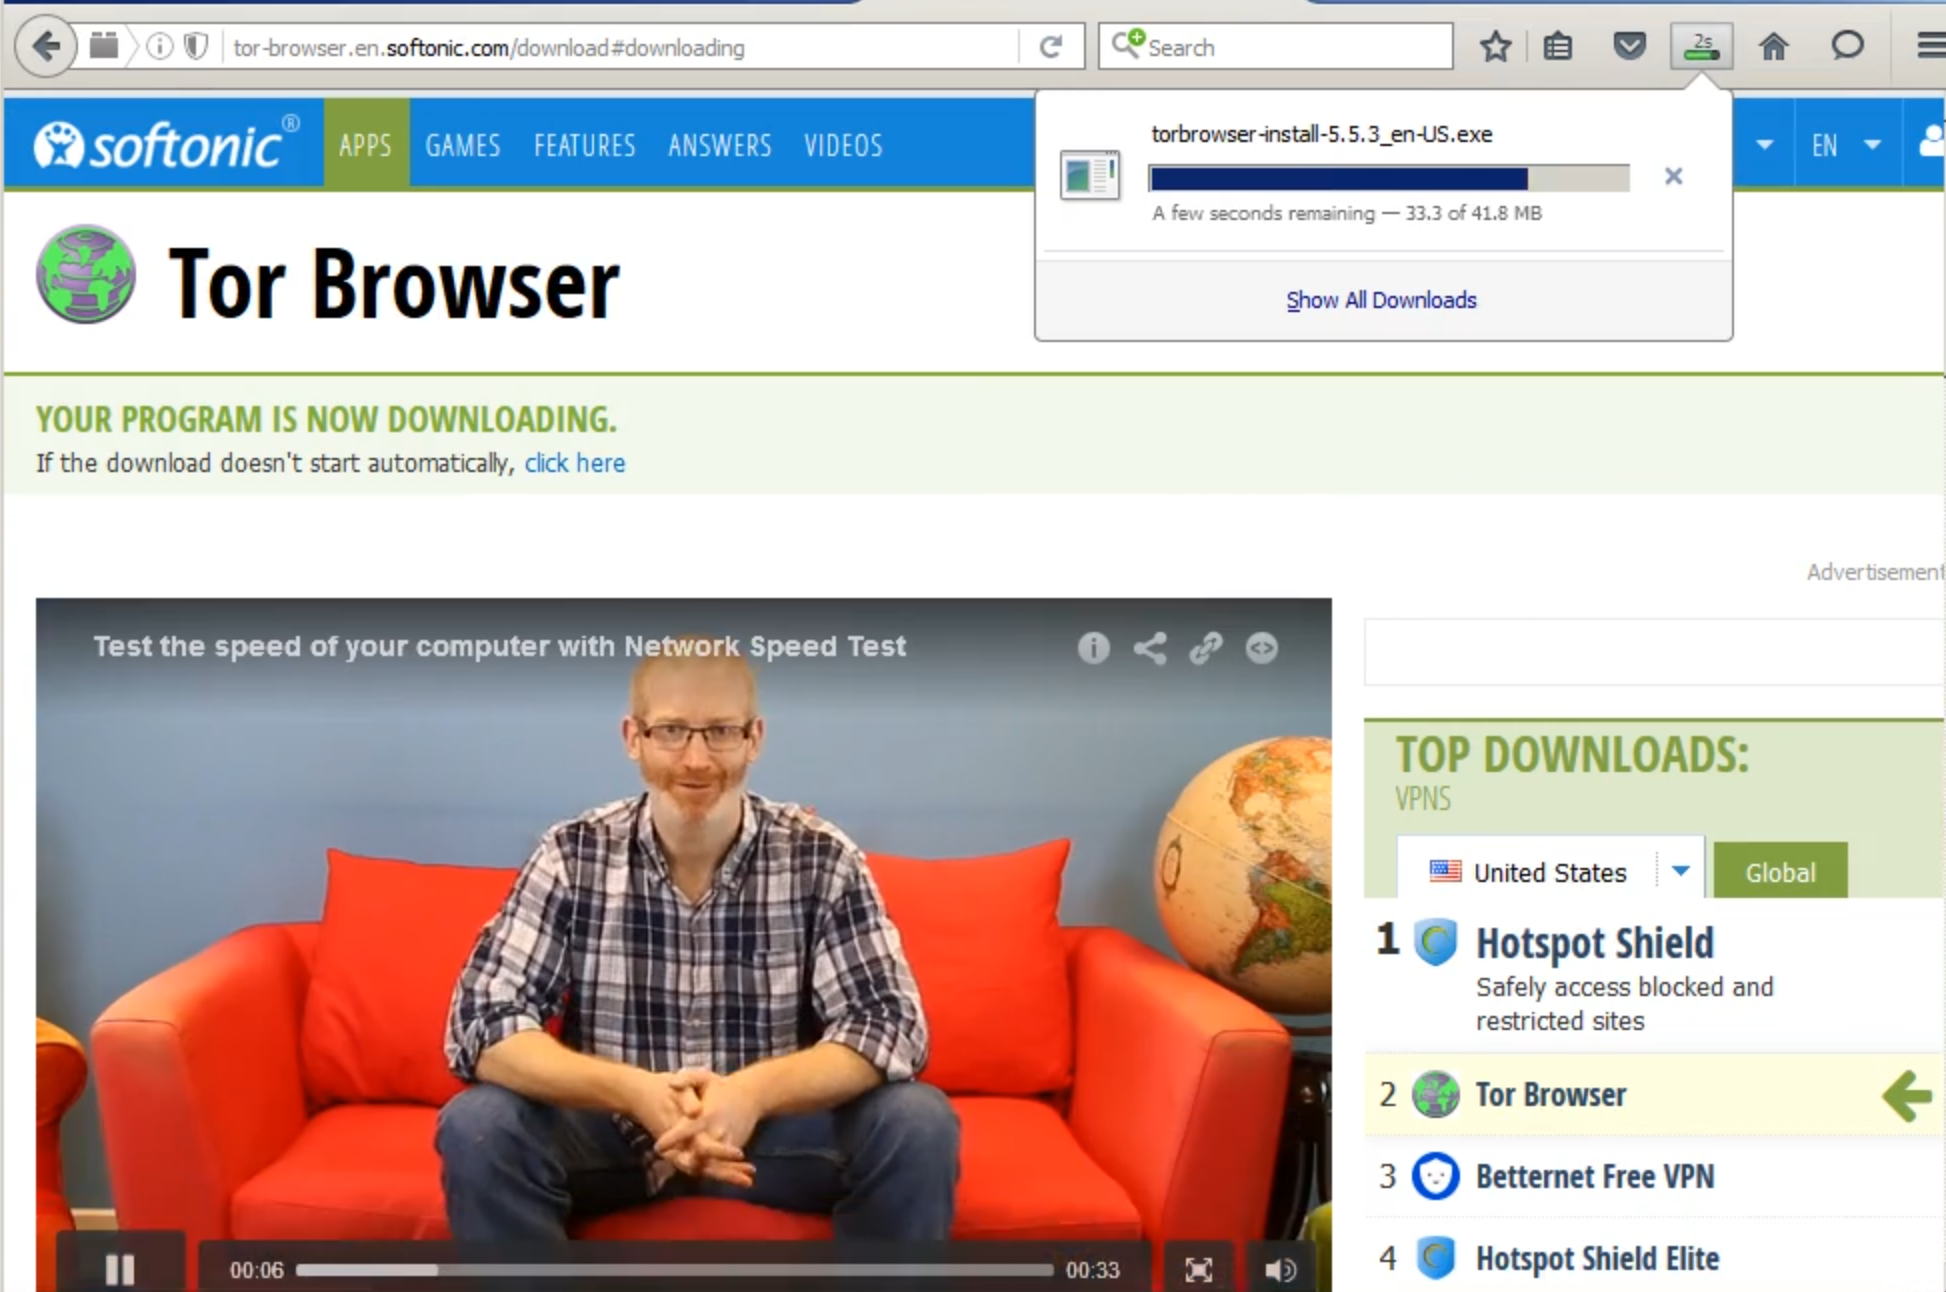
\includegraphics[width=0.5\textwidth]{../experiment/processing/bad-participants/20160330-161511-softsonic.png}
\caption{E3-NEW-X11-20160330-161511 downloaded Tor Browser from Softsonic, a reputable-looking but
unconfirmed site.}
\end{figure}



\end{document}
